%%%%%%%%%%%%%%%%%%%%%%%%%%%%%%%%%%%%%%%%%
% Masters/Doctoral Thesis 
% LaTeX Template
% Version 2.5 (27/8/17)
%
% This template was downloaded from:
% http://www.LaTeXTemplates.com
%
% Version 2.x major modifications by:
% Vel (vel@latextemplates.com)
%
% This template is based on a template by:
% Steve Gunn (http://users.ecs.soton.ac.uk/srg/softwaretools/document/templates/)
% Sunil Patel (http://www.sunilpatel.co.uk/thesis-template/)
%
% Template license:
% CC BY-NC-SA 3.0 (http://creativecommons.org/licenses/by-nc-sa/3.0/)
%
%%%%%%%%%%%%%%%%%%%%%%%%%%%%%%%%%%%%%%%%%

%----------------------------------------------------------------------------------------
%	PACKAGES AND OTHER DOCUMENT CONFIGURATIONS
%----------------------------------------------------------------------------------------

\documentclass[
11pt, % The default document font size, options: 10pt, 11pt, 12pt
%oneside, % Two side (alternating margins) for binding byhttps://v1.overleaf.com/20740335gynbkgcvnmvs# default, uncomment to switch to one side
english, % ngerman for German
singlespacing, % Single line spacing, alternatives: onehalfspacing or doublespacing
%draft, % Uncomment to enable draft mode (no pictures, no links, overfull hboxes indicated)
%nolistspacing, % If the document is onehalfspacing or doublespacing, uncomment this to set spacing in lists to single
%liststotoc, % Uncomment to add the list of figures/tables/etc to the table of contents
%toctotoc, % Uncomment to add the main table of contents to the table of contents
%parskip, % Uncomment to add space between paragraphs
%nohyperref, % Uncomment to not load the hyperref package
headsepline, % Uncomment to get a line under the header
%chapterinoneline, % Uncomment to place the chapter title next to the number on one line
%consistentlayout, % Uncomment to change the layout of the declaration, abstract and acknowledgements pages to match the default layout
]{MastersDoctoralThesis} % The class file specifying the document structure

\usepackage[utf8]{inputenc} % Required for inputting international characters
\usepackage[T1]{fontenc} % Output font encoding for international characters

\usepackage{mathpazo} % Use the Palatino font by default
%\usepackage[backend=bibtex,style=authoryear,natbib=true]{biblatex} % Use the bibtex backend with the authoryear citation style (which resembles APA)
\usepackage[backend=bibtex]{biblatex} % Use the bibtex backend with the 
%authoryear citation style (which resembles APA)

\addbibresource{Bibliography.bib} % The filename of the bibliography

%\usepackage[autostyle=true]{csquotes} % Required to generate 
%%language-dependent quotes in the bibliography


\usepackage{graphicx}
\usepackage{wrapfig}
\usepackage{pdflscape}
\usepackage{mathtools}
\usepackage{adjustbox}

\usepackage{listings}
\usepackage{color}
\usepackage{multicol}
\usepackage{amsmath}
\usepackage{mathtools}

\usepackage{verbatim}
\usepackage{amsthm}

\newcommand{\projectName}{CROSSMINER~}
\newcommand{\projectNameNoT}{CROSSMINER}
\newcommand{\cc}[1]{\multicolumn{1}{c}{#1}}
\newcolumntype{d}[1]{D{.}{.}{#1}}
\newcommand{\code}[1]{{\texttt{#1}}}
\newcommand{\codefoot}[1]{{\texttt{#1}}}

\newcommand{\CrossSim}{\textsc{CrossSim}\xspace}
\newcommand{\CrossSimA}{\textsc{CrossSim}}

\usepackage{xspace}
\newcommand*{\ie}{i.e.,\@\xspace}
\newcommand*{\eg}{e.g.,\@\xspace}
\newcommand*{\cf}{cf.\@\xspace}



\definecolor{dkgreen}{rgb}{0,0.6,0}
\definecolor{gray}{rgb}{0.5,0.5,0.5}
\definecolor{mauve}{rgb}{0.58,0,0.40}

\lstset{frame=tb,
	language=Java,
	aboveskip=3mm,
	belowskip=3mm,
	showstringspaces=false,
	columns=flexible,
	basicstyle={\small\ttfamily},
	numbers=none,
	numberstyle=\tiny\color{gray},
	keywordstyle=\color{mauve},
	commentstyle=\color{dkgreen},
	stringstyle=\color{blue},
	breaklines=true,
	breakatwhitespace=true,
	tabsize=3
}





%----------------------------------------------------------------------------------------
%	MARGIN SETTINGS
%----------------------------------------------------------------------------------------

\geometry{
	paper=a4paper, % Change to letterpaper for US letter
	inner=2.5cm, % Inner margin
	outer=3.8cm, % Outer margin
	bindingoffset=.5cm, % Binding offset
	top=1.5cm, % Top margin
	bottom=1.5cm, % Bottom margin
	%showframe, % Uncomment to show how the type block is set on the page
}

%----------------------------------------------------------------------------------------
%	THESIS INFORMATION
%----------------------------------------------------------------------------------------

\thesistitle{Supporting the development of complex software systems by means of 
	\\API function call recommendations} % Your thesis title, this is used in the 
%title and abstract, print it elsewhere with \ttitle
%\supervisor{Prof. Dr. Davide \textsc{Di Ruscio} \\ Dr. Phuong T. Nguyen} % Your supervisor's name, this is used in the title page, print it elsewhere with \supname
\supervisor{Dr. Davide \textsc{Di Ruscio}}
\examiner{abc} % Your examiner's name, this is not currently used anywhere in the template, print it elsewhere with \examname
\degree{Master of Science} % Your degree name, this is used in the title page and abstract, print it elsewhere with \degreename
\author{Claudio \textsc{Di Sipio}} % Your name, this is used in the title page and abstract, print it elsewhere with \authorname
\addresses{} % Your address, this is not currently used anywhere in the template, print it elsewhere with \addressname

\subject{Computer Science} % Your subject area, this is not currently used anywhere in the template, print it elsewhere with \subjectname
\keywords{} % Keywords for your thesis, this is not currently used anywhere in the template, print it elsewhere with \keywordnames
\university{\href{http://www.univaq.it}{University of L'Aquila}} % Your 
%university's name and URL, this is used in the title page and abstract, print 
%it elsewhere with \univname
\department{\href{http://www.disim.univaq.it/}{Department of Information 
		Engineering Computer Science and Mathematics}} % Your department's name and 
%URL, this is used in the title page and abstract, print it elsewhere with 
%\deptname
\group{\href{http://researchgroup.university.com}{The Software Architecture Group}} % Your research group's name and URL, this is used in the title page, print it elsewhere with \groupname
\faculty{\href{http://faculty.university.com}{Faculty Name}} % Your faculty's name and URL, this is used in the title page and abstract, print it elsewhere with \facname

\AtBeginDocument{
	\hypersetup{pdftitle=\ttitle} % Set the PDF's title to your title
	\hypersetup{pdfauthor=\authorname} % Set the PDF's author to your name
	\hypersetup{pdfkeywords=\keywordnames} % Set the PDF's keywords to your keywords
}

\begin{document}
	
	\frontmatter % Use roman page numbering style (i, ii, iii, iv...) for the pre-content pages
	
	\pagestyle{plain} % Default to the plain heading style until the thesis style is called for the body content
	
	%----------------------------------------------------------------------------------------
	%	TITLE PAGE
	%----------------------------------------------------------------------------------------
	
	\begin{titlepage}
		\begin{center}
			
			\vspace*{.06\textheight}
			
			
\includegraphics[width=0.2\linewidth]{images/univaq}
			
			{\scshape\LARGE \univname\par}\vspace{1.5cm} % University name
			\textsc{\Large Master Thesis}\\[0.5cm] % Thesis type
			
			\HRule \\[0.4cm] % Horizontal line
			{\huge \bfseries \ttitle\par}\vspace{0.4cm} % Thesis title
			\HRule \\[1.5cm] % Horizontal line
			
			\begin{minipage}[t]{0.4\textwidth}
				\begin{flushleft} \large
					\emph{Author:}\\
					\href{http://www.johnsmith.com}{\authorname} % Author name - remove the \href bracket to remove the link
				\end{flushleft}
			\end{minipage}
			\begin{minipage}[t]{0.4\textwidth}
				\begin{flushright} \large
					\emph{Supervisor:} \\
					\href{http://www.jamessmith.com}{\supname} \\% Supervisor name - remove the 
					%\href 
					%bracket to remove the link  
					\emph{Co-supervisor:}\\
					\href{http://www.jamessmith.com}{Dr. Juri Di Rocco} % Supervisor name - remove 
					%the 
					%\href 
				\end{flushright}
			\end{minipage}\\[2.5cm]
			
			\vfill
			
			\large \textit{Corso di Laurea Magistrale in Informatica}\\[0.3cm] % 
			%University 
			%requirement text
			\textit{}\\[0.4cm]
			%\groupname\\
			\deptname\\[2cm] % Research group name and department name
			
			\vfill
			
			{\large Academic Year 2017/2018}\\[4cm] % Date
			%\includegraphics{Logo} % University/department logo - uncomment to place it
			
			\vfill
		\end{center}
	\end{titlepage}
	
	%----------------------------------------------------------------------------------------
	%	DECLARATION PAGE
	%----------------------------------------------------------------------------------------
	
	
	
	
	
	%\begin{declaration}
	%\addchaptertocentry{\authorshipname} % Add the declaration to the table of contents
	%\noindent I, \authorname, declare that this thesis titled, \enquote{\ttitle} and the work presented in it are my own. I confirm that:
	%
	%\begin{itemize} 
	%\item This work was done wholly or mainly while in candidature for a research degree at this University.
	%\item Where any part of this thesis has previously been submitted for a degree or any other qualification at this University or any other institution, this has been clearly stated.
	%\item Where I have consulted the published work of others, this is always clearly attributed.
	%\item Where I have quoted from the work of others, the source is always given. With the exception of such quotations, this thesis is entirely my own work.
	%\item I have acknowledged all main sources of help.
	%\item Where the thesis is based on work done by myself jointly with others, I have made clear exactly what was done by others and what I have contributed myself.\\
	%\end{itemize}
	% 
	%\noindent Signed:\\
	%\rule[0.5em]{25em}{0.5pt} % This prints a line for the signature
	% 
	%\noindent Date:\\
	%\rule[0.5em]{25em}{0.5pt} % This prints a line to write the date
	%\end{declaration}
	
	
	
	
	%\cleardoublepage
	
	%----------------------------------------------------------------------------------------
	%	QUOTATION PAGE
	%----------------------------------------------------------------------------------------
	
	\vspace*{0.2\textheight}
	
	%\noindent\enquote{\itshape Thanks to my solid academic training, today I can write hundreds of words on virtually any topic without possessing a shred of information, which is how I got a good job in journalism.}\bigbreak
	%\hfill Dave Barry
	
	%----------------------------------------------------------------------------------------
	%	ABSTRACT PAGE
	%----------------------------------------------------------------------------------------
	
	%\begin{abstract}
	%\addchaptertocentry{\abstractname} % Add the abstract to the table of contents
	%The Thesis Abstract is written here (and usually kept to just this page). The page is kept centered vertically so can expand into the blank space above the title too\ldots
	%\end{abstract}
	
	%----------------------------------------------------------------------------------------
	%	ACKNOWLEDGEMENTS
	%----------------------------------------------------------------------------------------
	
	\begin{acknowledgements}
		\addchaptertocentry{\acknowledgementname} % Add the acknowledgements to the table of contents
%		The acknowledgments and the people to thank go here, don't forget to include your project advisor\ldots
		
		First, I would like to express my special thank to my advisor Prof. Dr. Davide Di Ruscio for his kind support and encouragement. He has been always open for any discussions, thus helping me advance my research.%suggestions and remarks.
		
		I am grateful to Dr. Juri Di Rocco and Dr. Phuong T. Nguyen for helping me during the time I performed the research as well as for proofreading my thesis. They have been responsive and supportive of me.% during the developing of my work.
		
		Finally, I want to express my very profound gratitude to my beloved family and to my friends who provide me with unconditional support and continuous encouragement throughout the years of my study. This work would not have been possible without them.
		
	\end{acknowledgements}
	
	%----------------------------------------------------------------------------------------
	%	LIST OF CONTENTS/FIGURES/TABLES PAGES
	%----------------------------------------------------------------------------------------
	
	\tableofcontents % Prints the main table of contents
	
	\listoffigures % Prints the list of figures
	
	\listoftables % Prints the list of tables
	
	%----------------------------------------------------------------------------------------
	%	ABBREVIATIONS
	%----------------------------------------------------------------------------------------
	
	%\begin{abbreviations}{ll} % Include a list of abbreviations (a table of two columns)
	%
	%\textbf{LAH} & \textbf{L}ist \textbf{A}bbreviations \textbf{H}ere\\
	%\textbf{WSF} & \textbf{W}hat (it) \textbf{S}tands \textbf{F}or\\
	%
	%\end{abbreviations}
	
	
	
	%----------------------------------------------------------------------------------------
	%	PHYSICAL CONSTANTS/OTHER DEFINITIONS
	%----------------------------------------------------------------------------------------
	
	%\begin{constants}{lr@{${}={}$}l} % The list of physical constants is a three column table
	%
	%% The \SI{}{} command is provided by the siunitx package, see its documentation for instructions on how to use it
	%
	%Speed of Light & $c_{0}$ & \SI{2.99792458e8}{\meter\per\second} (exact)\\
	%%Constant Name & $Symbol$ & $Constant Value$ with units\\
	%
	%\end{constants}
	
	
	%----------------------------------------------------------------------------------------
	%	SYMBOLS
	%----------------------------------------------------------------------------------------
	
	%\begin{symbols}{lll} % Include a list of Symbols (a three column table)
	%
	%$a$ & distance & \si{\meter} \\
	%$P$ & power & \si{\watt} (\si{\joule\per\second}) \\
	%%Symbol & Name & Unit \\
	%
	%\addlinespace % Gap to separate the Roman symbols from the Greek
	%
	%$\omega$ & angular frequency & \si{\radian} \\
	%
	%\end{symbols}
	
	%----------------------------------------------------------------------------------------
	%	DEDICATION
	%----------------------------------------------------------------------------------------
	
	%\dedicatory{For/Dedicated to/To my\ldots} 
	
	%----------------------------------------------------------------------------------------
	%	THESIS CONTENT - CHAPTERS
	%----------------------------------------------------------------------------------------
	
	
	
	
	\mainmatter % Begin numeric (1,2,3...) page numbering
	
	\pagestyle{thesis} % Return the page headers back to the "thesis" style
	
	% Include the chapters of the thesis as separate files from the Chapters folder
	% Uncomment the lines as you write the chapters
	
	
	
	
	
	
	
	
	
	
	\chapter{Introduction}
	\label{sec:Introduction}
	% !TEX TS-program = pdflatex


In recent years, the problem of API recommendations rises more and more in relevance in the complex software systems. When a developer writes some code to implement a specific features, he should want some suggestions about useful methods for the library that he is using. Nowadays, a project is not more implemented from scratch but, following the paradigm of software components reuse, developers typical use frameworks, tools, plug-in that make an intensively use of APIs. An API (Application programming interface) is a set of procedures, protocols and objects that gives to the developers the necessary building blocks to implement a specific functionality in easy and understandable way. Their variety depends on the language that the developer use and it usually composed by libraries with objects and methods necessary for the completion of task. This definition is very general and it may change based on the context of the developed project; so, the developer may get confusing about what kind of method or class to use or how to use them in a proper way. Moreover, many APIs are not well described and in many cases documentation miss at all. Although there are forums and dedicated website, as StackOverFlow, with well-organized topic and a lot of code examples, the developer looses its time to search the proper hints for a specific problem. Another aspect to take into account is the fact that each developer have its programming style and so a certain snippet of code could be useful for a user but meaningless for another one. 
\newline
A real big issue is how to perform a good enough recommendation in this context, balancing possible bias and putting the proper hints for the developer. Moreover, the form of the recommendation is also important because, in general, there are variety of possible suggestion such as code snippet, patterns for the methods, enhance documentation and all things that make a recommendation really usable for the current project. In this work, we focus on API function call and we propose a recommendation tool. This work is developed within the European CrossMiner project  ~\cite{https://www.crossminer.org/_nodate} and integrates some aspect related to the API recommendation domain. As overall aim, the project wants to monitor, analyze and extract data in the context of operative source software (OSS) environment. In this kind of system, there are issues and challenges to be addressed in order to reach a high quality projects, as the choosing of software components to be used during the development. The most difficult part in this task is the searching of the proper software component that is more suitable for the entire projects. Nowadays, the complex software system are really big and it is not so easy to select and deploy a component in the right way. Crossminer wants to face this problem trough various components that address a specific issue relate to the OSS domain, like:
\begin{itemize}
\item Source code analysis tools to extract and store knowledge from the source code of a collection of open-source projects;
\item Natural language analysis tools to extract quality metrics related to the communication channels, and bug tracking systems of OSS projects by using Natural Language Processing and text mining techniques;
\item System configuration analysis tools to collect and analyse system configuration artefacts;
\item Workflow-based knowledge extractors that simplify the analysis of a complex software system;
\item Cross-project relationship analysis tools to manage a wider range of open source project relationships, such as dependencies and conflicts, based on user-defined similarity measures and the creation of project clusters;
\item Advanced integrated development environments that will allow developers to adopt the  knowledge base and analysis tools directly from the development environment, that providing alerts, recommendations, and user feedback which will help developers to improve their productivity.
\end{itemize}
The figure below represents the Crossminer approach, including all issues addressed by the project:\\


\begin{figure}[H]
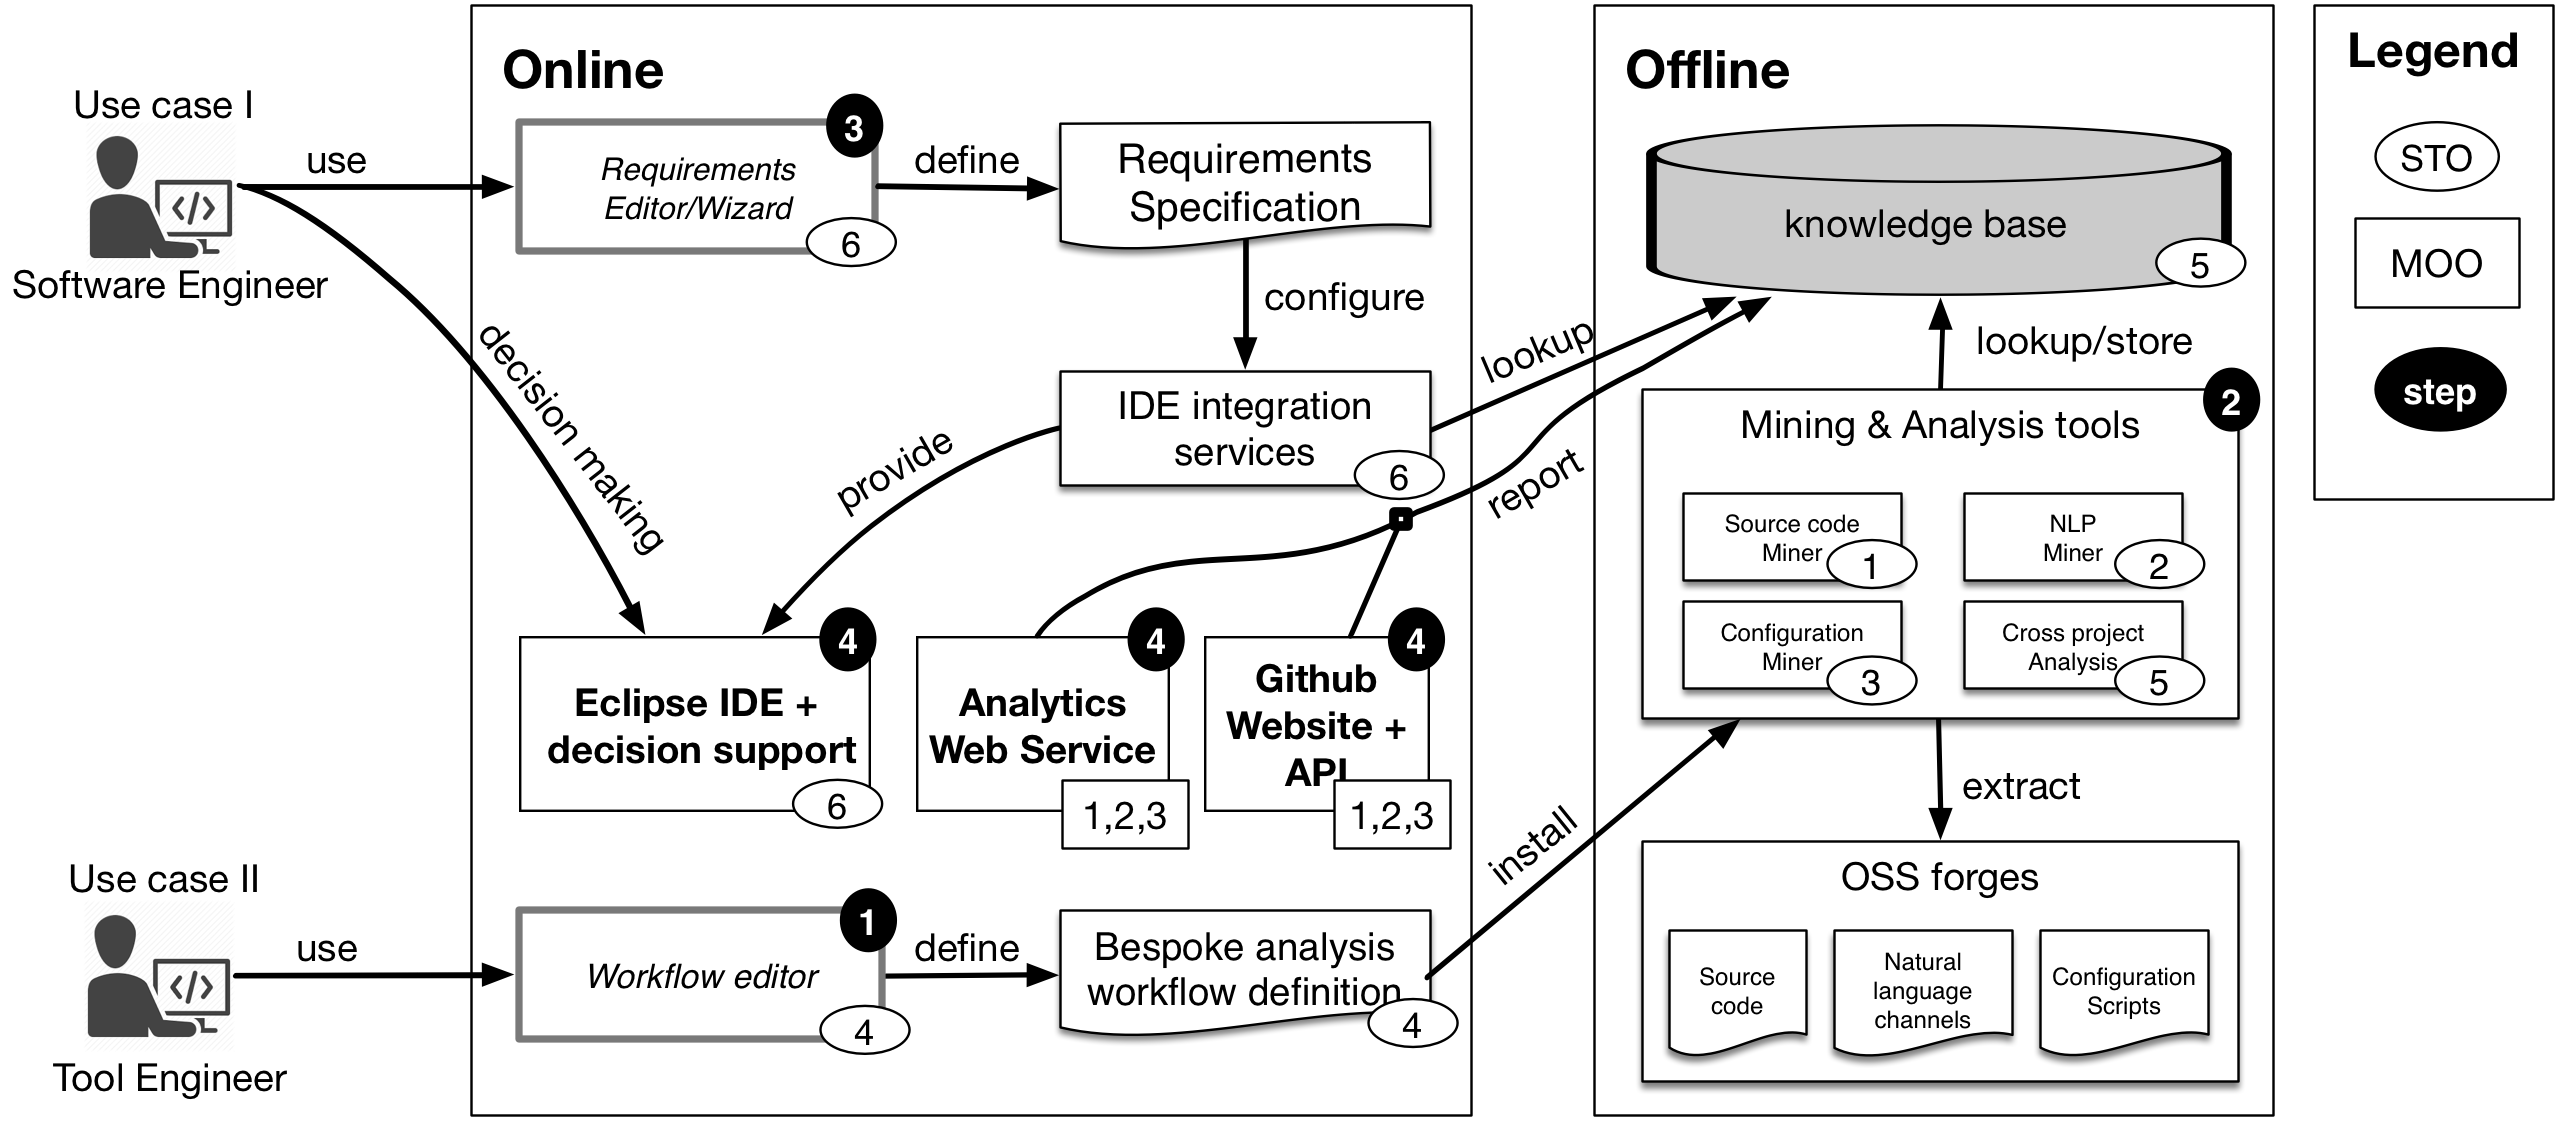
\includegraphics[width=14cm,height=14cm,keepaspectratio]{images/crossminer.png}
\centering
\caption{Crossminer approach}
\label{fig:cmd}
\end{figure}

Among all these challenges, the work presented in this thesis wants to propose a novel tool that perform API function call recommendations in the context of Java projects. It is integrated in the CrossMiner knowledge base component in a flexible way. The figure 1 represents the entire knowledge base; the proposed approach gives support for the APIrecommender subcomponent in the picture.

\begin{figure}[H]
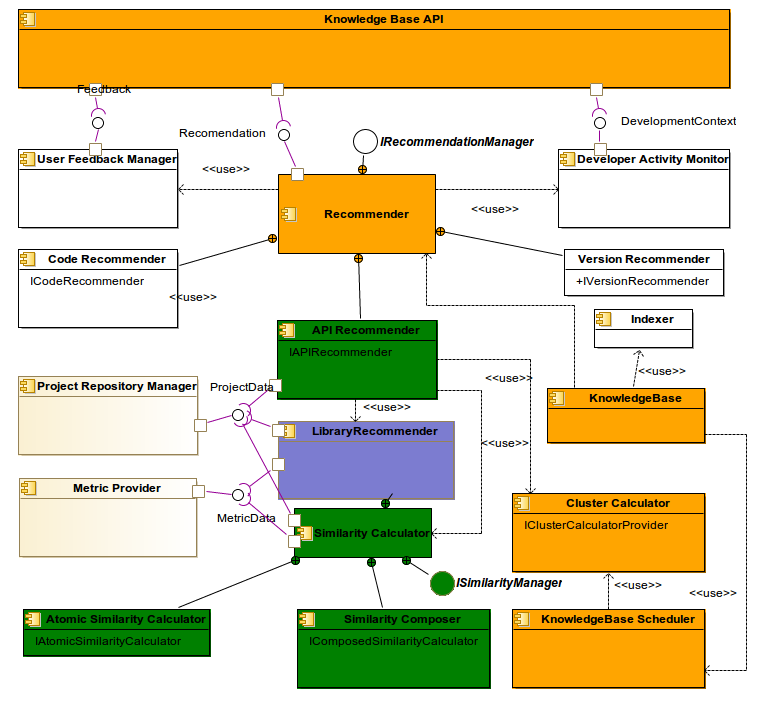
\includegraphics[width=12cm,height=12cm,keepaspectratio]{images/Kb.png}
\centering
\caption{Crossminer knowledge base}
\label{fig:cmd}
\end{figure}

	
In particular, we combine the concepts of code cloning and patterns to retrieve real code snippets that show a concrete usage of the libraries used by the developer. We choose this approach because code snippets represent immediate hints in the developing context, as a concrete usage of a method or class is more relevant rather than a JavaDocumentation description or the list of imports. We exploit also the code cloning technique in order to search and retrieve possible suggestion.\\
The work is organized in this way: in section 2 we provide a general overview on the key concepts used in the developed of the proposed tool. These concepts are the definition of API and recommendation; there are very general terms and the literature are plenty of examples and definitions in such a way that it is impossible to give an exhaustive overview. For this reason, we try to define in the right manner the context suitable for the proposed approach, by avoiding the perfect coverage of the topic and limit ourself to a few but relevant concepts for our aims. Moreover, we provide a general state of the art of the code cloning domain, with some definitions as cloned fragment, sources units and comparison algorithms. We also present different code cloner to have an overview on the different approaches and finally, we present Simian, the code cloner used in the proposed approach.
Section 3 gives an overall view of the problem, considering the most used and famous tool used for facing the API recommendation problems. They use very different techniques and a state of the art is necessary to better understand approaches, level of the recommendations and possible issues that arise when we develop these kind of systems.The general API recommendations procedure involves the visit of the AST, some clustering techniques and a ranking as postprocessing phase and we compare various existing approaches. Among these works, we select CLAMS for its results to perform our recommendations and PAM  for validate our approach. \\
The section 4 we describe the proposed tool that perform the final recommendations. It combines the results coming from CLAMS, inserted in the related works section, that are snippets of code representing patterns for a certain library. We use CLAMS as a black box component as it is written in Python (except for slight changes pointed out in the related section) to produce patterns for a library and then, we use Simian to analyze the developer's file, that contains what he is developing and, in particular, the fragment of code on which he wants the recommendations. As final results, the tool gives a novel patterns in form of snippet of code that contains method invocation and all useful variable to use them in the proper way. In the Section 5, we propose an evaluation framework based on AST of the code.The aim of this framework is to validate in an empirical way the produced recommendations by analysing the method declarations and invocations. To do this, we use JavaParser to retrieve the snippet of code that represent the context and Rascal a meta programming language to parse the AST of the developer's project in order to represent in the proper way the context, very important to evaluate if the suggested patterns are the correct ones for it. The evaluation is performed by considering four metrics: precision, recall, success rate and f measure. All the metrics are explained in the related section and it is used on the list of method invocations retrieved by Rascal. Moreover, we use PAM as to compare the final results. Finally, in the Conclusion section, we analyze possible future works in this area, starting from an improvement in the recommendation format and alternative techniques with respect to the code cloning used for this work.

	
	
	
	\chapter{Background}
	\label{sec:Problemdefinition}
	\subsection{Recommendation in complex software system}
First of all, we have to look at definition of recommendation.  In general, a recommendation is a suggestion or a proposal as to the best course of action, often provided by an authoritative body or expert domain. The key concept when we talk about recommendation is the context, because it changes meaning with respect to the type of system that a developer is working in. \\
We can find recommendation system in software engineering (RSSE) that gives the necessary information about suitable items for a software engineering task in a specific context. When a developer starting to work on a project, there are several information spaces, also called landscape, that describe all involved information in the overall developing process. In~\cite{martin_p.robillard_introduction_2009}, the authors define all possible information spaces in software engineering but this definition can be applied in whatever software complex system. Related to the developed project, the main definition is the project source code and project history, that give the context of developing. The project source code is useful to understand the structure of it, especially when we looking for method declarations, method calls and possible most frequent pattern while the project history tells something about the changing happened in the code from a older version to another. \\
This changes are usually captured by a VCS (version control system) although this kind of system isn't easily browsable and techniques like data mining or machine learning are required. Development environment also belongs to this information spaces classification and it includes all scripts, commands and tools used to test and run the system. Another big information space is defined by API that are linked to the project as well as their documentation, a good starting point to better understand their behaviours. Moreover, the authors consider also two types of traces when a user is developing a project: interaction traces, composed by the list of user's actions like search on website for particular component or interface and normally this kind of information are captured by an IDE (like Eclipse); the execution trace, instead, regarding the software runtime execution and the collected information are in general function calls and results of computation at every time. Finally, a very important information space is represented by the web that becomes more and more relevant in recent years; in particular, Stack Overflow questions and answers site is the most used by the developers as we can find a lot of concrete example about code snippets as well as information about interfaces, technologies and tools. \\
As we can see, all this information spaces represent an huge data mine and there are many problems to extract the correct information from it. First of all, the available information are heterogeneous and context awareness while a typical user is looking for a quickly solution related to its specific context. Furthermore, the complex software systems are rapidly growing and it can lead the overload information problem. So, looking at this problem, it is necessary to find a proper way to do recommendation, in the manner that the developer find a good solution in very few time without waste it to search in very large context. For the software engineering context, the authors propose RSSE, a recommendation system for software engineering based on capturing the context, giving the proper recommendation. The process involves some kind of data preprocessing, capturing the context, select the correct recommendation using collaborative filtering techniques and show them to the user.\\
 The first phase involves often effort because includes many type of operations on data like transformation, gathering, filtering, aggregation and so on. The next step is the capture of the context, that is a key issue in a recommendation system. In another domains, like e-commerce for example, the context is strongly related to the user's characteristics and its behaviours; reversely, in the software engineering and in the software domain in general, the recommendation are related to the task that the developer wants to perform. So, in this domain we talk about the task context, that in general a smaller part of the final solution. This kind of systems are called task-centric against the human-centric system in which the recommendations are related to the user. However, the capturing of this context could bring some bias, in particular we could be in the situation in which the context are extremely precise, maybe because we have a lot of information, but the user, especially if he is a not expert domain, doesn't known how to use them or how to provide enough information to describe in the proper way the context. After this preparatory phases, a recommendation algorithm can be executed to produce the final output. The literature is plenty of this techniques that go from the collaborative filtering techniques to similarity matrix, as we will see in next section. Of course, the choice of the algorithm to be used affects the precision, the accuracy and the coverage of the approach, making this task the most important during the development of a recommendation system. The last step is the presenting of the recommendation to the final user. Also in this case, the form of representation depends on the domain in which the recommendation system operates; so, considering the context, we can have a list of function calls, variables, classes as well as documentation or issues reports. Beyond the form of recommendations, a recommendation system must be to classify and rank the results, following a well-formed criteria, such as number of lines, probability, time, average rating and so on. This criteria naturally depends once again on the task context. \newline
Moving in the context of the IDEs, auto-completion can be a kind of recommendation at runtime because the developer, usually through shortcuts, wants suggestion for specific functions and methods. This technique uses often documentation embedded in the IDE (like JavaDoc in Eclipse) and it adapts itself  to the context, in this case the imported libraries in the project. Moving to a more general definition, we are in the query auto completion (QAC) domain, used in several contexts like search engine, as described in~\cite{DBLP:journals/ftir/CaiR16}.\\
It is a particular form of word prediction: when a user is typing something, such as fragment of code,method declaration or just first characters, QAC completes the query using different techniques like n-gram technique, probabilistic methodologies and heuristic learning algorithm. Beyond the used technique, QAC system ranks the possible results of a query following a predefined criteria. In case of auto-completion, the query engine maps the prefix, namely the query that the user is writing, to possible list of results and gather all the date in a effective data structure like prefix tree in order to avoid waste of time. Another purpose of a QAC system is try to predict the user's prefix, by retrieving the top rank queries before the entire process is finished. Moving to the possible approaches, there are two main categories: heuristic model and learning-based model. These two category can be divided again into three categories: time sensitive, contextual based and demographic-based. The first is involved when there are time constrains while the contextual and demographic based categories are strongly related to the user's previous history. \newline
So, we look at the different types of context that a recommendation system must face. Depending on the context, the proposed recommendations change too, sometimes in a radical way. For us, the context are represented by Java projects and in particular, API function call related to external libraries.

\subsection{Learning API: issues and solutions}
Moving on the concept of API, we have also in this case huge amount of definition in the literature and it's necessary to specify very well the context in we are. In general, an API (application programming interface) is defined as a set of procedures, protocols and objects that gives to the developers the necessary building blocks to implement a specific functionality in easy and understandable way. Depending on the context, these building blocks can be classes, interfaces and methods properly declared and used or intermediate software that acts as middleware in different situations as well as in the hardware context. The concept of API is strongly related to libraries that a developer uses and the kind of application that he is developing. So, we can have remote API to interact with different resources like databases deployed anywhere through protocol. \newline
Another issue is the complexity of an API, that depending on different factors like their structure and affect their usability, as pointed out on~\cite{martin_p._robillard_what_2009}. In this work, the author analyses the developer's difficulties when he wants to approach to an API; in particular, this work looks to the professional developers at Microsoft and try to understand what are the main issues in the API context. As starting point, the author of the article asks to a population composed by 30,000 people among engineers, developers and program manager in the Microsoft context. The survey starts with some questions about the developer's skills, to asses the knowledge of the participants. \\
Then, it contains questions about the problems on learning an API, strongly related to the context, familiarity with the application domain, the obstacles faced during the learning phase and so on. From the initial population, the author select 83 developers and compare the answers between the expert domain, like senior software developer engineering and lead software architects, with the novice and junior developers. From these results, he grouped in five categories obstacles that surface from these people during the learning phase in the API development. Among these, the category with the more answers is the obstacles bring to the absence or inadequate resources in the learning phase, such as not suitable code example, partial information about the content of APIs, no reference about the task to perform, inadequate resources format and insufficient high-level design and not well-formed structure of the API. Other problems are related to the structure, especially for debugging and runtime phases, the developer's background, technical issues and problems that arise during the runtime execution.\\
 In order to mitigate these issues, the documentation of an API must include good examples for the functions and code to develop, the support for case study scenarios, good organization of the relevant design elements. Another key point is the context, because the API change often their behaviour depending on it, as pointed out from 12 audio interview that author made with the developers adding their answer to the initial survey. In general, APIs follow the so called low barrier to entry, that consist to give just few information and key concept about the API structure and design, sometimes involving basic code examples. Although it is a very spread techniques, the survey underlines that is not enough to give a concrete help during the learning phase. Many developers involved in the survey, in facts, claim that they are often confused about multiple uses of a certain function, because there are different approaches to implement a feature but they not understand what is the proper one, considering also the context in they are. This issue affects also the general structure of the API, like the design that often generate confusion if it is not well specified and the survey respondents want also to understand what are the rationale behind the API.  \newline
Although the abstract design and the overall structure are important when we talk about the API usage, the most immediate and concrete hints are related to code example, as showed in the proper section of the article that we are analyzing. In particular, the survey shows that the Microsoft developers not always  understand the examples provided in the documentation, as they are not well documented or the authors of API not underline the purpose underlining a particular statement or function. The Table 2 shows the main three category of code example that could be provide by an online documentation or in a general readme file of the API. 
\begin{table}[H]

  \caption{ The three main category of code example }
  \label{Table:2}
\begin{adjustbox}{width=1\textwidth}

\begin{tabular}{|c|p{8cm}|}

\hline
 \textbf{Code example category } & \textbf{Description} \\
\hline
 Code Snippet & It gives just a flavour of basic concepts of the API and their possible use\\
\hline
Tutorial & It is a quite complete example of a possible use of API, with multiple methods and functions usage\\
\hline
Application & It gives a well structured example of the API, given also the development context \\
\hline
\end{tabular}

\end{adjustbox}
\end{table} 

Looking at these categories, the code snippet provides an immediate hint but is more related to a specific issue, such as opening a connection or initialize a particular object. The tutorial provides a more complete examples, with different methods, often followed by a textual explanation with the aim to show the rationale behind the code. The code example coming from the applications, instead, wants to give a general overview on the API features and it includes demonstration samples and complete open source projects. However, the Microsoft developers involved in the survey denote that usually the code snippet doesn't provide how to put together all the small pieces. Another problem is that the code examples on the Internet are out-of-date and the maintenance of them is still an opening question. The author, considering the answers coming from the survey, lists the possible improvements related to the code examples, by providing best practice in a certain situation, by giving the design behind the code example and by showing in a clear way how the API works in practice. All this information should be inserted in the documentation provided with the API.\\
Finally, the author of the survey analyses also the behaviour of an API, that sometime diverges from the declared one in the documentation or from the code examples. The developers suffers in particular for unexpected behaviours of similar components or methods, that varying from a context to another. Although this survey is conducted over Microsoft developers, it points out some key concepts when a user is approaching to learn and use an API, especially for the proper exploitation of provided functions.  \newline
Also in~\cite{by_christopher_scaffidi_why_2006}, the author underlines some issues and challenges when a developer is approaching to use and understand an API, such as the already mentioned inadequate documentation or the inappropriate abstraction in the overall design. The article suggests also possible workaround for the different situations that the API designers should take into consideration. The ideal design flow when a API designer should be follow includes the gathering of information from the stakeholders (mainly other developers that wants to reuse the API functionalities), map the requested features to the proper components and set up the glue code to make an usable and understandable platform. However, this implies a well specified design flow and a lot of time, and sometimes the timing constrains on the publication of a new API don't allow to have a complete and exhaustive documentation. \\
Also in the case of the Hello World examples, they are often not sufficient for the common user, especially if he is not an expert domain. Another potential problem is represented by the orthogonal functionalities, also called internal couplings. This term refers to the situation in which a method is strongly dependent with another or its behaviour can affect other parts of the system. To avoid these situations, an API's designer must keep the overall platform as simpler as possible, by limiting the exponential growing of the system. Concerning the abstraction problem, the users are in the situation in which the requirements don't match with the proper methods or interfaces provided by the API. This situation go beyond a lack of information in the documentation, because it is a problem that affects the initial design of the API. A designer should set abstractions for each user's requirement, in order to maintain the proper mapping and to avoid the loss of functionalities. Another possible solution is to use the facade pattern to make more accessible the API itself. The last main issue underlined in the article is the external dependencies, called assumptions, that an API could require to perform a certain operation. For the designer a possible solution can be the limitation of external calls to another API, maybe by reusing the internal API features. \newline
All these possible solution that the author provides in the article are inspired by three key concept. The first and most important is to make smaller the problem as possible, by splitting the initial one to little problems that can be solved in less time. Another strategy involves the approximation of the solution, looking first of all to the user's requirements and try to satisfy them. Finally, if the feature or the functionality to implement is really complex, an API's designer should choose an approach that is optimal in the average case. In this way, he reaches good results in reasonable time.\newline
As said before, the usability takes an important role in learning the API. In~\cite{marco_piccioni_empirical_2013}, the authors focus their attention on this problem, with a human survey similar to the one already analysed. In this case, however, they define two key concept and measure the usability of an API taking into account the so called cognitive dimension and usability token among the participants. The first one involves a cognitive framework based on the human reaction that take place when a user is implementing a particular feature specified by an API. This indicator wants to measure what is expected during the developing and what really happen. With this technique, the authors gather the reactions and so the implicit feedback coming from the programmers avoiding in this way the bias led by subjective perceptions. Of course, the cognitive analysis is combined with the classical research question, about the difficulties to learn a new API, the understandability of the usage and the abstraction of the overall platform. The usability tokens instead are extracted from the interviews to measure different developer's behaviours in different situation. Here below there are the list of the tokens used in the questionnaire:
\begin{itemize}
\item surprise: it measure the unexpected behaviour of a particular component of the API, that seemed different at the beginning;
\item choice: it evaluates the capacity of the developer to understand what is the optimal solution for solving a particular problem, like use the proper data structure;
\item missed: it belongs to the abstraction problem, when the developer loses something because he don't understand the API design;
\item incorrect: in this case, the developer uses in the wrong way the provided function or classes;
\item unexpected: this token describes the situation in which the user takes decisions that are not documented by the API's designer.
\end{itemize}
As we can see, the usability tokens are strongly related with the cognitive dimensions and they can combined with themselves to depict a particular situation in which some obstacles appears at the same time. The experiment is overtaken on ABEL, an object oriented library for storing and retrieving huge amount of information. The results of this empirical study, that involves heterogeneous group of developers, show that the critical issue is to understand the relations between types and classes, not always understand by the participants. Other minors issues are the incorrect usage of the provided interfaces or the treatment of constructors without arguments, but in those cases the developers are able to overshoot these issues. \\
So from these works, we can understand the difficulties in approaching an API, as there are many aspects to take into consideration. As we will see, for the our proposed approach we used code example and in particular the snippet of code to perform the recommendation, trying to avoid the above issues related to the API such as the lack of best practices and the ambiguous usage of a component. Another emerging aspect is that the documentation should be clear about the design, the abstraction and the features provides by the API. We don't directly work on the documentation, but we try to offers a solution at level of code that could be integrate this lack of information.



\subsection{Code cloning taxonomy}
To support recommendations, we choose an approach that involves code cloning analysis. When we analyze a software complex system, it is very easy to find duplicated lines of code, especially in case of very big projects. This situation are led by the copy and paste technique, very used in most of situation in which is necessary to save time or simply because it offers an easy solution to the current problem that the developer is facing. Although the copy and paste works in theory, it is not the better solution because the cloned code can bring some unexpected side effects on the other parts of the software and, anyway, it offers a solution only in the short term period. Although this behaviour is discourage in general, many techniques is based on find the clones without removing them. \\
The purpose of these tools, the so called clone cloners, is to analyze software complex system and find the common parts among them. During the analysis, it is also important to clarify how the code has been compared and what the word cloned really means. Two fragments of code could be declared clones also if their are not exact duplicated but even if they share the most of the structure (such as the variable name, the statement structure and method calls). So, a code cloning tool must be analyze also the structure, the AST and the token composition, plus the textual plain code of course. There are several techniques in the code cloning field and we look at~\cite{chanchal_k._roy_comparison_2009} to have a brief but clear overview on this topic. In general, a clone detector try to find the similarities between two fragment of source code. These analysis depend first of all from the level of details that the tool wants to reach: to make a very simple example, each code cloner could be set a different similarity function in order to set the level of cloning. They differs also in term of the comparison of two fragment of code, such as AST, textual comparison and so on. As we can see, there are a lot of concepts and techniques in this approach and to avoid get confusing, the authors create a very useful taxonomy to classify the activity of code cloning, showed in table 2.

\begin{table}[H]
 \caption{ Code cloner tools taxonomy}
 \label{Table:2}
\begin{adjustbox}{width=1\textwidth}
\begin{tabular}{|p{3cm}|l|}
\hline
\textbf{Code cloner type} & \textbf{Level of similarity}  \\
\hline
Type-1 & The code fragments differs only from the whitespaces, comments ad layout \\
\hline
Type-2 &  \vtop{\hbox{\strut Two code fragments that are syntactically equals}\hbox{\strut  except for the same conditions of type-1 plus identifiers, literals and name variables   }} \\
\hline
Type-3 &  \vtop{\hbox{\strut This kind of clone detector looks for variation (add, delete or change) in statement}\hbox{\strut that appears in the fragments, plus the previous conditions  }} \\  
\hline
Type-4 &  \vtop{\hbox{\strut We have this kind of cloner when the computation that the fragments}\hbox{\strut perform are equal without considering the syntactic implementation   }} \\
\hline



\end{tabular}

\end{adjustbox}
\end{table} 


Although there are a huge number of tools and techniques, there is a common clone detection process that it has to be considered in order to avoid very critical loss in time and spaces. In fact, even using whatever tool the computation became a big issue if the common part among fragments are unknown at the beginning of the process. So, the authors identify an overall process to approach the code cloning activity, even all the steps are not required depending on the situations. The preprocessing phase, first step, is necessary to discard useless elements in the fragments of code like embedded code that appears in some language and to obtain the source units. These units can be very different depending on the purpose of the cloner and sometime they can be partitioned again in comparison units, depending on the structure of the original source unit (the common case is when we have an if-else structure in which the comparison units could be the different branches). \\
After the preprocessing, if the code cloner go further the textual analysis, a transformation phase is required, to bring all the fragments to a common representation. Among the possible normalizations that we can apply to code fragments, we have the removal of whitespaces and comments, the normalization of identifiers (for example, through order sensitive index scheme), pretty-printing that affect the layout and structural transformation (for example, by removing the modifiers in a particular language). When we have a comparable units, a different comparison algorithm is run depending on the tool in order to obtain the list of matches. In this phase, we have to distinguish the fixed-granularity tools, in which the units that belongs to same block have the same granularity from the free-granularity ones in which the aggregation continues until a threshold value is reached. The list of candidates for the comparison are usually source coordinates that must be map on the original source code files. The last step is a post-processing in which clones are ranked or filtered depending on the aim that the tool wants to reach. This phase can be done by human evaluator or through a parametric heuristic algorithm. The picture below summarizes the entire procedure:\\

\begin{figure}[H]
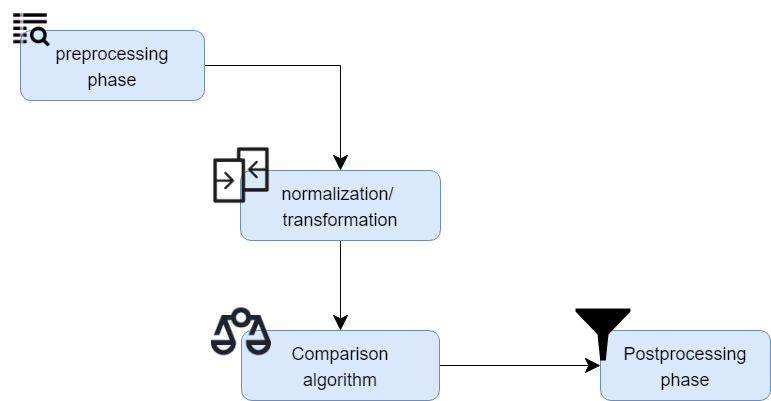
\includegraphics[width=14cm,height=14cm,keepaspectratio]{images/codeCloning.png}
\centering
\caption{Typical code cloning phase}
\label{fig:cmd}
\end{figure}

Looking now to the different tools, most of them rely on different approaches to identify cloned code. The most immediate approach is the textual one, as the transformation and normalization phases are often very slight. The tools that implement this approach use fingerprints or substring of the source code. The fixed lines that are used in the comparison are called window and they are encoded with a hash function. To obtain fragments with different lengths, the tool apply simply a slicing on the window. The lexical approach, instead, works on the tokens obtained from the source code through the compiler-style lexical analysis. This technique is more robust because it avoid the whitespaces and other dirty code that we want to exclude from the comparison. The big issue of this approach is that it not consider the syntax; so, the founded clones may overlap different syntax units but preprocessing or postprocessing can avoid this situation, like pretty-printing techniques to format the code in a better way.\\
 Go further, we now look at the syntactic approaches, that usually rely on the AST of the code. There are two main process  that we can apply: the tree matches and structural metrics. The first relies only on the AST extracted from the code and the comparison takes place on the subtrees. Each element of the source code(variables, literals) became a leaf of the tree and subtrees that are hashed into buckets in order to reduce the number of comparisons that take place in each bucket. However, the complexity of this approach is very high and recently there are code cloner that try to mitigate this drawback by serialize the AST as node sequence in order to reach the same speed in the same way of  token based techniques. The second approach  exploits the AST is based on structural metrics. This technique avoid the direct comparison between ASTs by collecting a vector of metrics, usually calculated through fingerprints functions that consider classes, methods and statements for the metrics. The last approach that we look is the semantic technique that relies on static program analysis to provide more information rather than the syntactic one. With respect to the other approaches, the source code is represented by a PDG (Program Dependencies Graph) to keep trace the data dependencies among expression and statements. So in this case, the comparison of the clones turns to the problem of finding isomorphic subgraphs. Finally, in the literature we can find hybrid approaches that involves both syntactic and semantic analysis. \\
This work includes also a very useful tool comparison, in which the authors show a list of code cloners and their main features. This state of the art is done by taking into account several parameters and metrics, like availability of the tool, IDE integration, comparison algorithm, kind of granularity, pre or post processing, language support, subsystem, possible empirical validation and overall complexity. However, it is not easy to evaluate code cloning tools, because there are several factors and hypothesis to taking into account when we do the comparison. As we have seen, each code cloner have its own techniques, comparison algorithm, approaches, complexity and supported languages, so the risk to do an unfair comparison is concrete. To avoid this situation, the authors set a list of possible scenario that analyze different kind of situations in which the code cloning activity may be useful. \\
The evaluation analyzes the results and if the considered code cloners are able to detects the common part in particular duplicated snippet of code. There are two type of scenario that the authors consider in the evaluation: the first type is more technical and it considers the changes at the level of code, taking as example functions that implements some features. The second type of scenario involves more a not expert domain user and it focuses on the intentions rather than directly on the features. For the first type of scenario, we have several functions that implement a very simple mathematical operation. By the copy and paste activity in which literals, variables and statement change from one scenario to another, the authors look for the code cloners that are able to detects these changes. Some scenarios also take into account the changes that happening in the code like addition or deletion of lines of code. In the second scenario, instead, a user claims the functionality that he wants to realize or how many clones in the code the cloner found. 
\newline
\subsection{Code cloners: techniques and features}
After the code cloning taxonomy, useful to give a general but exhaustive idea about the code cloning domain, we show some code cloners that use interesting techniques to solve the problem of first track the cloned code and thus retrieve the results to the developer. Among the these techniques, we are focusing on the string match one, as it is closer to the code snippets used in our approach. The detection of cloned code is a complex task, that can be bring different issues and criticisms. As pointed out on~\cite{stephane_ducasse_effectiveness_2005}, there are key points to take into account we are looking at the string match code cloner. First of all, it is necessary to avoid false positive, the part of code that is marked as duplicated but should not be, and false negatives, that appears when the code cloner is not able to detect the cloned code during the analysis. \\
Moreover, the scalability takes an important role in this task, because the code cloning tool must analyse complex software system that are exponentially growing in recent years. An strongly related issue is also the analysis of multiple languages: a good code cloner, in facts, should be able to recognize the cloned code beyond the different syntaxes and lexical differences among the different programming languages. Then, the authors propose their approach, based on the lexical analysis, following the Bellon's case study about the code cloning. In this framework, the author categorizes the clones into three types: the exact clones (Type 1), the part of code that differs from each other for the identifiers (Type 2) and clones in which statements or expressions have been inserted, deleted or changed (Type 3). This case study provides also a measure to detect how a clone is far from an other, in term of the distance. Before proceeding with the tracking activity, the authors make also the so called noise elimination on the source files that contain the cloned part to find. The noise elimination, according to the implementation done by the authors of the article, is similar to the token normalization mentioned in the taxonomy part: they remove all black spaces, comments and blocks that are not useful for the comparison.
This phase is necessary to avoid false negative. Once they have done this normalization, they can apply the string matching techniques, based on a line by line comparison in which they look for duplicated code. From their experience, it is very difficult to find an exact code, following the definition of the Bellon'work; it is most probable to find the duplicated code among the code fragments with some modification, like insertion or deletion of statement, variable and so on. \\
Finally, the apply some filters on the results, as the single line is not enough to be significant for the cloning analysis. Therefore, they set two metrics, one related to minimum length sequence of the duplicated part, and the second related to the maximum gap size, measured between two compared sequences. To improve the recall of the results, they also set up a second normalization based on regular expression and they test the overall approach on the same dataset of Bellon's study, composed by the Cook and Weltab application. 
\\
Another interesting approach for the code cloning is showed in~\cite{nils_gode_incremental_2008}, in which the author proposes a code cloner with multiple revision of the code. In this way, the analysis takes place not only on the original code but also on the fragments already processed, in order to give a more accurate analysis. For this purpose, he develops the IDA tool (Incremental detection algorithm). It is based on tokens, a sequence of characters with a collective semantic, and on suffix trees, already mentioned before. In particular, for the token the author use a multiple token table as data structure, in order to avoid the problems that arise during the multiple revision task. In facts, during the analysis tokens already analyzed by the tool must be discarded from the next phases and this could be left holes in the table, with a consequent overhead in the basic operations like the access to data. So, when a new fragment of code is analyzed, a related token table has been created to speed up the operation. Also the suffix tree is affected by these side effect and the IDA tool uses a generalized suffix tree to solve these issues. \\
\newpage
In this version, the suffix tree has multiple strings instead of one. The main advantage is the speed of the operations like deletion or update of a single leaf. Similar to the token tables, the fragment of code already analyzed is deleted from the tree. Considering also the clone pairs, IDA integrates all these components in order to make the multiple revision of code. The process starts with a preprocessing phase in which IDA sets up the necessary data structure in and reads the source files from the directory. Once this initial phase ends, the tool starts to build the token tables and the corresponding edges and nodes in the suffix trees when it is processing new files; reversely, it deletes the nodes of external edges that represents the deleted files. The approach is tested on three open source software, wget for downloading files, gcc compilers and the Linux kernel. \\
The last example that we show is related to Cren~\cite{jablonski_cren:_2007}, a code cloner specifically developed for IDEs. In particular, the author set up our tool for Eclipse platform, going further with respect to the related Eclipse features, like refactor or  find and replace. The issues to face in this field are mainly related to copy and paste that the a typical user do to integrate into an IDE another methods or function. Reversely with respect with other approaches, that use heuristic algorithms often very complex, the authors of Cren provide a simpler but  effective solution in the IDEs context. 
The core of the approach is represented by a tracking of cloned part, followed by consistent rename of variables, that is the typical behaviour of a developer when he tries to reimplement an API component. By exploiting the JDT features related to the AST of the code, Cren is able to find not only the cloned pairs but also a clone groups, represented by a sequence of two or more elements. Variables and identifiers that share some characteristics are inserted in a same group. Once it found the clones, it can show to the user what are the cloned part in the context and, thanks to Eclipse interface, it is able to highlight the cloned pairs that change dynamically with respect to the context. \\
In this way, the user can refine also the search of the cloned parts, as Cren keeps trace about the cloned part already founded. Cren represents an interesting mix between the code cloning technique and the IDE context. After this overview about the taxonomy of code cloning and some examples of code cloner, focused in particular about the suffix tree technique and an incremental code cloner, we will see in the next section the code cloner chosen for the implementation of our proposed approach. 
\newpage
\subsection{Simian overview}
As we see from the introduction, we can perform recommendation at different levels of abstraction (pattern, documentation, code snippets) in order to give a complete and useful hints to a developer. In our approach, the overall idea is to perform the API recommendation at the level of code snippets that represent the patterns related to the developer's file. To do this, we can exploit the code cloning analysis that we present in the previous section. As tool for this approach, we choose Simian, a project developed in Java that performs this kind of analysis for many languages as Java, C, C\#, Ruby, JavaScript, COBOL, Lisp, SQL, Visual Basic. Following the taxonomy in table 2, we can define Simian as a Type-2 code cloner with flexible options on variables, literals, modifiers and it performs the analysis following the textual approach described before. All possible options are described in table 3, although we discard some options that are related to languages different from Java, like ignoreRegions for C files. \\
To test the main functionalities of the tool, we can simply run the jar file a available on the website~\cite{https://www.harukizaemon.com/simian/_last_nodate} by specifying options and the input file. As output, we see on the console the textual representation of source coordinates that describe the number of duplicated lines and the original source files. The results are showed on the console. Notice that we can change the type of output using the formatter option (in table 3). 
Following the tool classification already mentioned, Simian has this following features: 
\begin{itemize}
\item It supports object oriented and web languages;
\item It not require additional tools or dependencies;
\item It is language and platform independent;
\item It has free granularity and it analyze line by line of the source files;
\item It uses fingerprints technique for the code representation;
\item It applies transformation on variable, types and literals using options.
\end{itemize}
Among the main drawbacks, Simian not include IDE supports and we must do a manual integration that we will see in next section. Moreover, it not includes some preprocessing or postprocessing phases as well as an heuristic algorithm for the threshold or an aggregation phase at the end of the process. It has no external dependencies and it is free downloadable but empirical evaluation is not available. Also the algorithm complexity is not well define, although it depends first of all by the number of lines of code and on the website there is a time approximation for one comparison. In particular, Simian is able to find 141,070 duplicate lines of code in 2,406 files in less than 5 seconds, that means about 28 lines of code for each second. 



Table 4 describe a very simple scenario in which we pick four pairs of Java project with the description of their main features and how lines of code are in commons.

\begin{center}
\begin{table}[H]
  \caption{ Simian options used in the experiment }
  \label{Table:3}
\begin{adjustbox}{width=1\textwidth}
\small
\begin{tabular}{|l|p{4cm}|p{6cm}|}

\hline

 \textbf{Option name} & \textbf{Default value} & \textbf{Description} \\
\hline
 -threshold & 6 &This option fix an lower bound on the number   of duplicated lines of code (if present)  \\
\hline
-formatter &  none , possible values: plain, xml, emacs,    vs (visual studio), yaml, null &   This option is used to obtain results in a specified format\\
\hline
-reportDuplicateText & disable , type + to add &   With this option, the duplicated lines of code  present in all projects are printed on the console    \\
\hline
-language & disable , type + to add &  This option specify the  language of the input files to compare   \\
\hline
-defaultLanguage & disable , type + to add &   If not file type is not specified, Simian inferred the type and set it as default    \\
\hline
-failOnDuplication & able , type - to remove & If this option is able, it causes  an exception when the checker finds duplicate code     \\
\hline
-reportDuplicateText & disable , type + to add & With this option, the duplicated lines of codepresent in all projects are printed on the console    \\
\hline
-ignoreRegions & disable , type + to add & It ignores block in regions structures (only for C\# programming language)  \\
\hline
-ignoreBlocks & disable , type + to add &  It excludes specified blocks  from the comparison (start/end line must be specified  \\
\hline
-ignoreCurlyBraces & disable , type + to add & The curly braces are ignored  so it should be match as duplicate line \\

\hline
-ignoreIndentifier & disable , type + to add &   With this option, the variable with different identifiers match as equal  \\
\hline
-ignoreIdentifierCase & able, type - to disable &  This option not consider the case of identifiers  present in the code: so Name and name are considered equal \\
\hline
-ignoreStrings & disable , type + to able &  This option consider all strings  in the comparison and  doesn't take care about the form in which are write\\
\hline
-ignoreStringCase & able, type - to disable & Same as previous option   but consider the upper and lower case as the same \\
\hline
-ignoreNumbers & disable, type + to add &   This option considers different    numbers as equal  \\
\hline
-ignoreCharacter & disable, type + to add &    With this option, all character type match as equal  \\
\hline
-ignoreCharacterCase & able, type - to disable &  Same as ignoreStringCase but consider char by char. Useful for more precise analysis \\
\hline
-ignoreLiterals & disable, type + to add &   All literals should be seen  as equal for Simian  \\
\hline
-ignoreVariableNames & disable, type + to add &   This option allow to Simian  to see different variable names as equal \\
\hline
-ignoreModifiers & able, type - to disable &   This option doesn't consider modifiers of methods  (public, private, protected as element of  diversity in the code)\\
\hline



\end{tabular}

\end{adjustbox}
\end{table} 
\end{center}



\begin{center}
\begin{table}[H]
  \caption{ Projects considered in the comparison }
  \label{Table:4}
\begin{adjustbox}{width=1\textwidth}
\small
\begin{tabular}{|l|p{5cm}|p{3cm}|}

\hline
 \textbf{Projects name} &  \textbf{Main features}  & \textbf{Similarity level (duplicated LOC)}  \\
\hline
 ADTPlugin, ModiscoPlugin   &  Plugin projects created with same wizard & 39 lines of code in common\\
\hline
CyberGea, NeoEMFExample &   Very different projects that realize different features & No lines in common\\
\hline
CyberGea, Scuna project & The projects share only database part & 12 lines on common  \\
\hline
Simple Servlet, ServletSession &  Web projects with servelts & 35 lines of code in common  \\
\hline
\end{tabular}

\end{adjustbox}
\end{table} 
\end{center}

From the scenario, we can see that similar project share more line of code, like the first two pairs that are both Eclipse plugin projects. It happened because these projects are built with the same wizard procedure and share the initialization phase of the plugin, such as the activate method. The second pair of projects, instead, doesn't share any lines because the CyberGea project is another plugin projects that uses Mqtt paho client and JDBC libraries mainly while the Neo EMF project is related to construct a metamodel with the aim to create a Neo4j database. Then, we compare Cybergea with another project developed in this university, the Scuna project that involves Swing framework and the MySql library for java. Notice that in this case, the two project shares only this latter part and the lines in commons are very few. \\
The last example is related to Java Servlet in the web context and Simian analyze two kind of servlet, one without the handling of session and the second with this features. The tool is able to detect that there are many lines in common, as the servlet shares the initialization part in commons like the doGet and doPost methods. Notice that all the projects showed in this simple comparison are developer in the context of university projects and their aim here is only to show an example of the code cloning activity of Simian. As an additional remark, for this comparison we use the default options for Simian and launch it from the console, again just to give the taste of the kind of analysis that we will perform at deeper level for the proposed approach. \\ 
Before to go in deep in the explanation of our approach, we present now existing approaches that face the problem of API recommendations, considering different techniques and contexts.
	
	
	\chapter{Mining APIs: an overview of existing approaches}
	\label{sec:RelatedWorks}
	Considering the state of the art, there are several approaches that face the 
problem described in previous section. The key point is to find a simple and 
effective way to extract API functions call and build a recommendation system 
able to provide developers with very suitable recommendations with respect to 
the developer context. Even though several techniques and tools have been 
proposed over the last decade, most of them share the main activities shown in 
Fig. \ref{fig:apiRecommendationExistingApproaches}. In particular, the 
developer context consisting on source code files is analysed to obtain 
corresponding ASTs. The retrieved abstract syntax trees are taken as input by a 
similarity analysis step in order to retrieve from the available knowledge the 
cluster of API client source codes that share some similarity with the code the 
developer is working on. Subsequently, a ranking activity is performed in order 
to finally recommend the developer with source code fragments that on one hand 
are similar to the developer context and on the other hand permits to grasp how 
other existing projects use the considered APIs. In the following, 
representative approaches implementing the process shown in Fig. 
\ref{fig:apiRecommendationExistingApproaches} are presented and compared at the 
end with respect to a set of specific characteristics.




%So far, we have seen several approaches to perform recommendations related to 
%API context. The proposed tool from the literature are very different from the 
%point of view of dataset, similarity measure and clustering techniques but 
%they 
%share a conceptual model that starts from the abstract syntax tree of the code 
%to the final recommendations. This procedure is depicted in Figure 1, that 
%describe at high level the main steps to reach the final output. Many of these 
%are optionally but, as we have seen in the previous discussion, are strongly 
%recommended to perform a better analysis and to have good enough results.
%For the proposed approach, we choose to combine the results coming from CLAMS 
%with the code cloning technique, by using Simian. Basically, we propose 
%something that is different from the existing approach analyzed. For example, 
%we avoid to use clustering techniques because we rely completely on Simian for 
%this task.  

\begin{figure}[!h]
	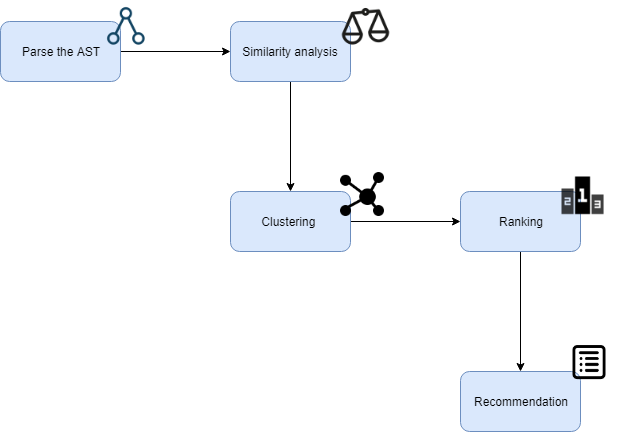
\includegraphics[width=12cm,height=14cm,keepaspectratio]{images/approach.png}
	\centering
	\caption{Main activities shared by existing techniques to provide 
	developers with API recommendations}
	\label{fig:apiRecommendationExistingApproaches}
\end{figure}






%To this end, several approaches are available able to 
%analyze the developer source, to adopt some similarity metrics, and to 
%optionally apply clustering techniques for representing the obtained results 
%in 
%the form of recommendations that should be clear and effective. 

%approaches that follow the same main skeleton to solve the problem; what is 
%different among them are the techniques, algorithms and produced results but 
%they are all useful and give the flavour of the API call function problem. 



\section{API mining framework: MAPO}
In~\cite{zhong_mapo:_2009} the authors propose MAPO that perform methods extraction using data mining techniques, clustering them to have a more representative data and build a recommender through GEF tool. So, they divided the process into three main steps: analyzing the source code, the API miner and API recommender. First of all, MAPO parses the source code coming from Java Github projects that use Eclipse Graphical Editor Framework (GEF), using JDT parser utilities that allow to analyze in deep a Java file and extract classes, interfaces, method invocations and method declarations. For the recommendations, MAPO considers as API method suitable for the recommender only those belong to third-parts libraries, considering the GEF framework as external, class cast and creation associated to external class and the method call that belongs to external class; basically, the authors ignore the libraries and so the internal API of the JDK. Then MAPO collects all source code by using @ as initial mark to identify a method call and \# as separator between method and related class. \\
This format is called ARFF and we will explain it in the related section. About the conditional statements, such as if, while and so on, the authors not considered the possible relations among multiple conditions and in practice the represent them as flat code in which MAPO considers all branches. As claim by authors, this simplification is necessary otherwise the mining phase is infeasible and the API recommender is not effected by them. Once the method calls are selected, there is the problem of method overweight and common-path overweight that involves respectively several method calls and sequence in common in the source code that can introduce bias in the result; for example, in fragment of code MAPO can select a method call only because it is replicated and not for its real effectiveness. To avoid this problem, the authors select the longest sequence in common that covers also the smaller sequence of method call and, in this way, the reduce the bias. Moreover, MAPO selects only third-parties libraries using inline methodology, that consist to explore the parse tree of classes and identify the ancestor and so excluding the JDK methods. \newline
Once MAPO have all method call, the next step is mining the sequence to produce recommendation. To do this, is not enough to consider all method sequences because this can bring incorrect results. So, MAPO using first similarity metric, based on the name and the usage of methods to identify similar sequence and then clustered them by using data-driven hierarchical clustering. In particular, the authors consider three level of similarity given by class names, method names and called API method and obtain in this way the similar sequence. Then, by using Mathlab tool, MAPO performs classical hierarchical clustering to obtain the ranked list of representative sequences, transform them into transaction and put them into a database. Finally, the API recommender is a Eclipse plugin that allow developer to click on the method of interest, execute a query on DB to show possible uses by using sample code and developer can also see details on the proper window tab in which the API method are highlight.\\
 To validate this approach, the authors use a dataset composed by 20 projects that used Eclipse GEF, run the tool and show the effectiveness of their approach by a quantitively comparison. To reinforce the validity, they also conduct an empirical study on by considering a set of tasks to do and select a group of Java developers that is involved to solve those tasks.


\section{Mining succinct API usage patterns: UP-Miner}
A similar approach is performed by~\cite{wang_mining_2013} in which the authors create UP-Miner tool that improve MAPO in term of accuracy. Going in deep, the aim of the authors is to achieve the succinctness but also the effectiveness of mined pattern that represent an enhancement of previous approach. Once the authors define API usage mining, that is the optimal number of patterns under a given threshold, they propose a clustering technique based on BIDE algorithm. As first step, UP-Miner extracts API pattern sequences using Roslyn AST parser from the projects that compose the dataset. Then, the apply the SeqSim n-gram technique that takes two sequence computes the similarity that is based on the shared items between them in term of objects and classes used and on the longer and consecutive sub-sequences rather than the shorter ones. This phase produces weighted results that are used for clustering that are conservative on, in sense that the maximum distance between two cluster is the maximum distance between two elements of those cluster.\newline
Then, UP-Miner use BIDE algorithm, that have the key concept of frequent sequence: a general sequence became frequent if its super-sequences (namely the sequences that contains the considered sequence) is greater or less of the given threshold. Consider this, BIDE algorithm can extract the longest common sequence that are useful to divided the results into different clusters, but it is not sufficient because at this point there may be some redundant cluster. So, it is necessary to apply once again the previous phase considering the cluster as usage pattern and this two-step clustering grants an improvement in term of redundancy considering also two different threshold (one for pre-BIDE and another for post-BIDE application). Until this, UP-Miner address the problem of coverage but the aim of the authors is to reach also the succinctness of patterns. To do this, UP-Miner use a dissimilarity metric that measure the diversity of a usage pattern from another and an utility functions to maximize in order to obtain the better results, decreasing the threshold at each step of the algorithm implemented for this task. \\
Once UP-Miner computes the correct and more succinctness as possible usage API pattern, the authors show them to the developer by building a probabilistic graph in which each node is a usage pattern and the edge is weighted with certain probability. To produce this prototype and make some experiments that involves the developers in a similar way as we see in MAPO, the authors use a very large C\# dataset as input files and compare their results with MAPO ones.

 


\section{Summarizing API with clustering techniques: CLAMS}
Go further with the examination of the existing approaches, we have also CLAMS tool proposed in~\cite{katirtzis_summarizing_2018} that follows a quite similar approach but it differs from the point of view of the results. In fact, CLAMS produces as API recommendations snippet of code that represents a pattern for a certain library. As usual, the preprocessing phase is done by analyze the AST of the source code (in case of CLAMS, projects related to 5 popular Java libraries) with a depth-first search using JDT as previous example. This phase produces snippet of code that brings all information about API implemented in the code. The similarity technique is based on Longest Common Subsequence (LCS) and is more effective rather than an analysis at source code level. By using this technique, CLAMS creates a distance matrix that is used as input by the clustering module of CLAMS, that implements the hierarchical version of DBSCAN algorithm, called HDBSCAN, plus a post-clustering processing to eliminate the sequences that are identical to snippets for each cluster obtained. The aim of HDBSCAN is to isolate the less representative methods and, more in general, points into a distribution that are really far from the rest of the dataset. \\
To do this, the algorithm uses a distance called core distance to draw a circle on the points to exclude and then computes the mutual reachability distance that reduce the presence of sparse node in the dataset. Then, by applying Prim's algorithm, HDBSCAN calculates the minimum spanning tree among the closer nodes and finally sorts them by a hierarchical clustering (this phase is not present on the original DBSCAN algorithm), as well explained in the related work. There is also a useful Python library used in CLAMS that provides utility functions to make all this step in a very understandable way. The core module of CLAMS is represented by the snippet generator, that performs six main steps in order to obtain the final snippets that represent patterns. First of all, CLAMS replaces all literals present in the code with their abstract type by using srcML, a tool that produce XML file starting from a source code, and removes all comments. At the end of this step, we have code with the same structure of the original source file but more abstract.\\
 Then, CLAMS identifies API call in that code and what are not related to them and creates two lists. In the next step, the authors identify all variable in the scope of the API sequence. To finish the process, the non-API statements are removed and they put on top of snippet variable declaration related to API, plus of course the snippet of code related to those API. So, the snippet of code that is produced in this way is composed by a sequence of variables related to API class and a possible use of them, with considering also the statements present in the original code (CLAMS retained also the structure of the code). The authors put a comment Do Something in the section of code in which the founded variables may be used. \newline
Once CLAMS has these results, the snippet selector module finds for each cluster the most representative snippets by giving them a score. To do this, 
the authors use another algorithm that works on AST, called AP-TED that creates a distance matrix between two clusters and from this, calculate the similarity. Finally, CLAMS ranks all representative snippet using the definition of snippet support define as follow: a snippet is supported if there is a file that contains a supersequence of it. An example of extracted pattern is depicted below and it is related to Twitter4j, a library that allows connection with a twitter client. 
\begin{lstlisting}
{
    AccessToken accessToken;
    final String CALLBACKURL;
    RequestToken requestToken;
    SharedPreferences prefs;
    Twitter twitter;
    twitter = new TwitterFactory().getInstance();
    twitter.setOAuthConsumer(OAuthConsumer.CONSUMER_KEY, OAuthConsumer.CONSUMER_SECRET);

    if(!prefs.contains(string) | !prefs.contains(string)) {
        try {
            requestToken = twitter.getOAuthRequestToken(CALLBACKURL);
            String authUrl = requestToken.getAuthorizationURL();
            // Do something with authUrl
        } catch (TwitterException e) {
            Toast.makeText(this, e.getMessage(), Toast.LENGTH_LONG).show();
            Log.e(string, e.getMessage());
        }
    } else{
        accessToken = new AccessToken(prefs.getString(string, string), prefs.getString(string, string));
        twitter.setOAuthAccessToken(accessToken);
    }
}
	
\end{lstlisting}

Moreover, for human readability reason, CLAMS beautifies snippet using A-style tool, that removes useless spacing and fixes the indentation of the final snippets. For the evaluation task, the authors use 5 popular Java libraries coming from Github projects and they are Apache Camel, Drools, Restlet framework, Twitter4j, Project Wonder and Apache Wicket. In the evaluation section of their paper, the authors taking into account different clustering algorithm and make experiments with HDBSCAN, already mentioned, k-medoids that is similar to the previous one but achieve more coverage but less precision. This algorithm is based on find a central point that has the equal distance from the rest of the point, called medoid. \\
In our case, the medoid is a particular method API call that is the most representative for the library. K-medoid algorithm uses also n-gram based technique and similarity distance matrix as HDBSCAN. To answer to the research question, the authors of CLAMS preform also a comparison with NaiveSum and NaiveNoSum approaches, that are clustering techniques less precise with respect to the HDBSCAN and K-medoids. In fact, the better results are coming out from the latter algorithms. \\
Furthermore, the evaluation is composed by a user survey about the utility and real support given by CLAMS patterns. All this information are available at the CLAMS official site, that contains also the Github project, the original dataset and the instruction to set up the environment to launch CLAMS as standalone platform on Linux machine. As claimed by authors, this work is really interesting and flexible because it is not dependent on a specific program language. The only constrain regarding the srcML tool to produce the XML files related to API patterns, but it is not a big issue from the adaptation point of view, as we can see later.



\section{API recommendation with statistical learning: APIrec}

APIrec tool~\cite{nguyen_api_2016}, instead, uses statistical techniques in order to keep trace of the context in which a developer writes its own code, by analyzing the co-occurrences and fine-grained code changes. Differently from the previous approaches, the authors keep trace of the context in which the API method call may be useful. As usual, to extract the source code from the 50 Java projects randomly selected from Github, APIrec navigates the AST of the source code using GumTree tool. Before going in deep with the implementation, the authors give several definitions that are useful to understand the behaviour and the contributions to the state of the art given by APIrec. \\
First of all, the term API for the authors indicates both external and internal method calls and APIrec performs recommendations only if the context of API is correct for a certain situation. Regarding the AST, we have the atomic change that represent a new element on AST composed by kind of operation, AST node and label. A collection of atomic changes is called transaction and is stored in a bag, a particular data structure that we commonly find in the AST definitions. An important concept that is a key definition for the APIrec implementation is the code context, represented by code tokens related to the API that the developer is writing. Taking into account the tokens, the authors consider both the distance and the order of this, as an API method calls have a specific call order and they are really effectiveness only if there are called in the proper way. To remark this feature, APIrec gives also a weight based on how near the token by is considering the distance matrix. Once they define this set of metric and concept, the authors show the inference model based on likehood scores taking into account both change of the context and code.\newline
The entire model is based on the correlation between a code token and another, expressed as we said in term of atomic changes in the AST and transactions. In particular, APIrec evaluates the probability that certain events, namely the transactions, occurs given another. This score is called association score and it is used to calculate the distance between two changes into the code as well as new methods that will take a part in the final recommendation. \\
At the end of these computations, all possible scores and weights are calculated but it is not enough to perform the recommendations. In fact, it is necessary to apply machine learning techniques in order to train APIrec with the code changes and context. To do this, the authors use hill-climbing adaptive learning filled with three parameters: numbers of co-occurrence founded with fine-grained atomic changes, numbers of co-occurrences related to changes tokens and two weights. With this process, the necessary scores are calculated and APIrec is able to perform the recommendation by considering the most probable method calls for a certain API. The methods are also ranked by highest probability of usage but also distance, scope and dependency are considered in the ranking phase. To support their tool, the authors conducts several experiments over a very large dataset, including also analysis regarding code change context, user empirical studies, evaluation of accuracy and predictions.



\section{Synthesizing API usage examples: Buse-Weimer algorithm}
Paper from Buse and Weimer~\cite{buse_synthesizing_2012} is still about API call but is focused to produce automatically a documentation for the projects in a human readable format.
Once they obtain data from mining phase, the proposed algorithm extract API pattern and rearrange them in a more readable and effectiveness format. The focus of this work is on Java documentation that provides useful hints and suggestions when a developer is implementing an API functionality. Although in general the Java doc helps in this kind of activity, it often lacks in something, as the examples are too general or it not able to give a concrete hint for the problem that the developer is trying to solve. So, the aim of the authors is to produce an enhanced version of documentation that is really useful for the developers, starting from retrieve the API patterns, defined as the sequence of function call for a certain API class, called target class. \\
Once this first step is done, the algorithm tries to produce a human-written documentation for the API, taking into account some characteristics such as the lines of code, that are 11 on average but 5 for the median. Moreover, the authors consider also the abstract initialization, abstract usage and exception handling. All this information is extracted using JDK utilities and they are validated by the authors, putting more effort on the human aspect. To validate the results, they involve over 150 developer and collect their answers about the proposed results. By analyzing these statistics, a typical developer wants multiple uses for a certain class or API method and not only one, that may be not useful for his particular context. Another key point is the conciseness of the suggested snippet of code, as well as the readability and variables names that must be related to the context, also including temporary ones to improve the readability. So, from this survey, we can identify four key points to achieve the human-written documentation: size of the code, readability, representativeness and concreteness.\newline
To reach these goals, we can look to the algorithm implementation, that the authors divide into four main step: the path enumeration, predicate generation, clustering and finally the output documentation. Starting from the path identification, they scan the code and identify acyclic part of the code that represent a path for the target class. Notice that this approach can led some bias but it happens in practice and the authors choose to stay close with respect to real implementation. \\
So, they use intensively human users to perform test and to measure the accuracy of their proposed algorithm. As the previous approaches, they parse the code and cluster the significant result with a distance matrix in order to build the related documentation. As the purpose is different from previous works, they are adding some clustering also on predicate and represent the abstract pattern as a graph. Then they compute symbolic execution over these paths on order to produce inter-procedural path predicates that are logical formulas used to represent the code and in particular, if a certain statement is reachable or not. From this abstraction, the algorithm computes use seeds that are local instantiations of fields, objects and whatever is related to the target class. Finally, from these it produces concrete uses, the real hints about the target class, that are stored in graph form in which edges keep trace about what happens before and so, in this way, we have the context as well as the chain of methods necessary to implements the features related to the target class. \\
To have better results, however, it is not enough to produce usage examples, as we seen so far with the other related works. Clustering is necessary to avoid heavy computation, and the proposed algorithm exploits the well-known k-medoids algorithm with some modifications, as the original algorithm is not suitable to detect distance about objects. The distance matrix that is taking into account by the k-medoids algorithm is based on the happens before relation obtained from the graph. So, at the end of this computation, the algorithm obtains the cluster and summarize them into abstract uses, represented once again in graph form. \\
The final step of the proposed algorithm is to produce the documentation. Starting from the abstract uses, it uses a topological approach to avoid the cycle and branches that appear in the code, as the final recommended documentation about the target class must be a flat file. Using this approach, the authors are able to retrieve a Java documentation related to the target class and respect also the Java syntax, so they avoid malformed documentation. Moreover, with this approach, the algorithm handles the exception treatment with try catch clauses, that are put always in the correct order. As said before, the focus of this approach is on readability of the recommendation from human's perspective, so the authors set up a very big evaluation framework composed by 47 SDK classes ads dataset, the eXaDOC tool as concurrent approach and over 150 people as tester. The threats rise up from this evaluation are related to the validity of dataset (it may be not indicative and it doesn't represent all possible situation) and the background of the developers chosen for the evaluation (not expert in the field). However, this approach is useful to understand the concept of readability in the API recommendation domain.

\section{Mining patterns for Android  API: APIMiner}
In  ~\cite{borges_mining_2015}, the authors extend APIMiner tool with API pattern considering Android projects from Github as dataset. In particular, they develop a module that perform the recommendation based on mining. The original API miner tool~\cite{montandon_documenting_2013}  retrieves information about the documented API method in the Android interface similar to JavaDoc view. This kind of recommendation coming from  concrete source code extracted from private repositories. The overall  architecture is composed by the source repositories, a pre-processing module based on slicing algorithm, the ranker module that classifies the summarized methods  considering all the lines of  code (source code metric), the number of commits in the original repositories (called process metric) and the number of download (called usage metric). \\
Moreover, the authors use also Java Weaver, a tool that builds and retrieves automatically the Java documentation related to the extracted methods calls. About the slicing algorithm, that represent the core of the system, it works as follows: first, it takes as inputs the API method call that the developer wants to analyze and all the body statement in which this method was found. Of course, this kind of analysis is performed off-line to avoid loss of time. At each iteration, the algorithm looks for similarity by analysing the list of variables present in the body statement of each method. If it founds some similarities, it put the method in a list that represent the final recommendation, as in this list there are the most relevant methods. The slicing is performed both backward and forward; the first looks the writing variables while the second analyze the the reading ones. The dataset is composed only by Android projects because this system provides an API to validate APIMiner approach. All the projects are under open source license and are compilable, otherwise the slicing algorithm doesn't work (it visits the AST to retrieve information about method calls). \\
Concerning instead the extension mentioned before, the authors perform the API extraction by considering FP-Growth association as main index of similarity and run it using Weka tool that consider also the relation between two API call, defined as sequence of methods that implements specific functions. This approach relies completely on Weka implementation. During the mining, the tool discharges the call with single call because is not relevant. The results are evaluated by define two main metrics: support, defined as the number of patterns that include the method, and confidence, the probability of the method in the antecedent transaction. The final recommendation is displayed in the JavaDoc window in Eclipse and Android Studio, although the results is related to Android API functions. With respect to original APIMiner work, the authors also extend the graphic interface in which the recommendations are showed; in particular, the tool shows the complete chain of method calls related to the client method. An important drawback of this approach is that it works only for Android projects and it is no tested at the moment for other kind of APIs.

\section{API usage pattern recommendations with object usages}
Then, we have a look on~\cite{niu_api_2017}, that perform clustering by using graph format. The authors, starting from a graph representation of the so called object usage, build a social network based on the co-existing relation among nodes. The aim of this work is to cover the less frequent API pattern in Android context. Before going in deep to the proposed implementation, the authors point out some definitions that are used in the approach. First of all, take a general code snippet, an object usage is a list of methods that belongs to an API class that are used in the part of code that we analyze; in general, a fragment of code can contain more objects usage and this feature is represented by a co-existence relation among objects usage. \\
So, one object usage became a node in the graph and, if there is a co-existence relation, we put an edge between them and the weight are the number of co-occurrences. An usage pattern, instead, is the sequence of object usages that belong to different API class. Once they define this to key concept, they underline the challenges underlying the API mining and propose an approach quite different that we have seen so far. In facts, the represent the object usage, and more in general usage patterns, with a graph as we said; then, they define the co-existence relation and method call similarity, that are the baseline to define a similarity score among API call. Regarding the co-existence relation, it is represented as a weight in the graph and represent the number of occurrences of the object usage in an API class; basically, objects usage that are included in a particular API class are connected by a co-existence relation. As the authors want to reach quite good coverage of API call and avoid the redundancy, they need some clustering technique, as we know from the other related works. \newline
To do this, the exploit the previous definitions and propose two level of clustering, one related to co-existence relation and the other one based on method calls similarity. For the first level, they propose a modularity index applied to community structures, defined as subnets of node densely connected. So, exploiting the graph format, they apply a greedy algorithm that calculates time by time the modularity, with the function goal that try to achieve the maximum one. By running this algorithm, they get the optimum cluster and perform the first level of clustering. For the second level, they focus on the method call similarity and propose the Gamma index, based on consistent and inconsistent comparison. A comparison is consistent if the distance of two object usage that belongs to different clusters is smaller than another pair that belong to the same cluster. By applying these two techniques, they obtain a good coverage of usage patterns and avoid the redundancy by using abundance metric that describes how many times an object usage appears in the corpus. Through this metric, the authors retrieve the most popular object usage but it is not enough to perform the recommendations. \\
The last step, in facts, is to map the objects usage into usage patterns in form of real code snippet that support the developer during the API implementation. For the testing phase, the authors provide a large corpus of 11,520 Android projects coming from Github, focusing on the Android Application Package (APK) because it contains the compiled code and it is not possible to analyze the Google Play original source code. The next step is the setup of a golden set that is a set of queries suitable to the author's purpose. This set is extracted in order to reach the high coverage as possible. The tool is fed with a single query and following the described process, the authors retrieve the expected pattern for that query. To validate the overall process, they also set up an user evaluation with questions about the readability and understandability of the suggested code.

\section{Automatic recommendations from feature request: Jira platform}
In~\cite{thung_automatic_2013}, the authors propose a tool for mining API and make recommendation within the JIRA platform, that is an issue management project based on summary, description and component related to a particular issue. The main idea of this work is to analyze the pre-change and post changed files and, in this way, find recommendations starting from a textual description of the input. The first step is the preprocessing of the input, necessary to clean the code and to give it a proper representation for the algorithm used in next steps. \\
This textual preprocessing is done taking into account two issue: tokenization and stemming. The first one involves the process of break into smaller piece of code the entire document using delimiters as frontier and put it in a word token structures (also called bag of words). The stemming, instead, is related to the root of the word and transform it in stem word: in this way, the authors summarize multiple words to avoid bias during the analysis. Once this preprocessing is done, the algorithm uses a term frequency indicator to count the number of times that a word appears in the document and so, obtain the most popular token. A similar measure is calculated also for the document and after a formula showed in the paper, the authors retrieve weights and put them in a vector; in this way, each bag of word is associated to a weight that measure its relevance for the recommendation. \newline
The framework is composed by three main part: history based recommender, descriptor based recommender and the integrator that put all together. For the history recommender, the algorithm compares the indicator on the Jira platform using similarity distance matrix, starting from Jira fields, named This module consider summary and description as key value of comparison and store them in its knowledge base called Historical Feature Request Database. Once the similarity scores are obtained, the algorithm perform aggregation of these scores and perform the final comparison between the historical scores (calculated in this step) and the new feature request that is coming. To do this, they create a top-k request looking at the history and choose the recommendation with the highest value among them. Description based component, instead, compares the new feature request with the Javadoc of the method, to have a more detailed recommendation. \\
Then, there is a preprocessing phase regarding the API doc which consists in extract method call taking into account the @param and @return annotation plus the discharge of HTML tags and Java comments. As similarity measure, in this phase they use cosine similarity between the current feature and the preprocessed API. The last component is the integration, that merge the historical part with the description part, apply Gibbs sampling and try to calculate the best results at each iteration. In particular, they pick first the no-zero historical recommendations and then compare them with the results of descriptor module; from these results, then algorithm creates a top rank recommendation related to the developer's features. \\
Regarding the evaluation of these results, the authors select 5 most famous Apache projects (Hadoop, CXF, AxisJava, Hbase and Struts 2) and looking for Github projects that implements these libraries. They filter these projects considering the presence or not of the pom.xml file and, after this preprocessing, they retrieve 207 projects as corpus of the tool. To select the golden set, the authors also considering the status of the file that belongs to Jira platform: in particular, they take into account is the new files are added or are changed with respect to original while they not include the deleted files to the golden set.


\section{API recommendation with reuse conducive development environment: CodeBroker}

Now we analyze CodeBroker tool, proposed in~\cite{ye_reuse-conducive_2005} that use information retrieval techniques in order to make recommendations. The authors consider a lot of techniques for their tool, such as information delivery, retrieval by reformulation, knowledge augmentation and finding task with similarity metric. All these definitions compose the conceptual framework that is a baseline for the implementation and evaluation of the CodeBroker tool. It is a interface agent with back-end utilities that takes a query as input and return the component related to it. Notice that this recommendation is based on Javadoc generate from Java source files. \\
The tool is based on two communication channels with the developer that is interested in API recommendation: one is an implicit where the system autonomously retrieve methods information and details from a given query. In this case it shows information organized in three layers, namely task relevance, signature details and full JavaDoc. Regarding the second channel, it is explicit because the developer can refine the query based on its current needs and the system can adapt itself to this new situation and this technique is called retrieval by reformulation. Furthermore, CodeBroker creates a discourse model to represent the projects and an user one to represent in some way the software knowledge and personal information regarding used method in the project. It uses LSA as similarity techniques to do comparison and Java core libraries as dataset to test the tool. About the implicit communication, this term describes a set of information that can be inferred by the system without taking in account the user's hints; for the explicit channel communication, instead, the tool considers the user's need by looking its model plus the discourse one mentioned before.\newline
As first step, CodeBroker arrange the query taking into account the context of the developer, called constrain part, the program that is the concept of functionality and the code that is the embodiment of it. So, for the similarity analysis, the authors consider the context and so the conceptual similarity and also the constrain similarity, that involved between two different signatures of the methods. About this last concept, they reuse it to apply the Latent similarity analysis (LSA) as main technique to perform comparison between two different API methods. Going in deep, the tool performs the so called signature matching that outlines the similarity of two components based on their signature structure. Although this comparison should be not representative enough, the authors claim that is suitable for their purpose: so, the value of the comparison is in the range from 0.0 to 1.0, that represent the exactly match between two different method. However, this first analysis must be enhanced by retrieval by reformulation technique as the LSA cannot analysis in deep fragment with comments or task relevant information from the code. So, as mentioned before, the authors use explicit communication channel to allow the developer to formulate once again the initial query: the typical use case is that a user want to improve the initial query with other components and so he change the query in order to retrieve more information or very different components with respect to the initial one. It is true especially for the Github repository, that have very complex structure inside them and may a no expert developer want to know all these details. \\
At this point, we can introduce the concept of module, namely the part of the code that implements the developer's main feature. This kind of activity is performed by building the discourse model of the developer, that represent the sequence of tasks necessary to implement the all features and it is used to improve the final components recommendation. At the beginning, this model is empty as the developer is starting to develop and he doesn't know at the beginning what are the components that are useful for his task. During the query phase, this model is filled with respect to the developer's choice and all this information are retrieve on the RCI console used for the final recommendation. There is another model that CodeBroker takes into account during its analysis: the user model, that represent the developer's knowledge in abstract form. \\
Based on this definition, it is very different with respect to the discourse model and it is partially filled based on the developer skills. This model is used to remove possible components that the user already known and so to avoid the redundancy problem. The authors define the knowledge as the number of implemented class by the developer and, in general, it is different from user to another. The final recommendations is performed through RCI-display already mentioned, with three layers: the first one shows the components related to the query, the second is linked to mouse movement (it displays signature information about the retrieved components) and, finally, a completed description in HTML external page, included the JavaDoc, belongs to the third layer recommendation. For the evaluation task, the authors use Java 1.1.8 core libraries and JGL library, with 663 classes and about 7000 methods to analyze. 

\section{Mining API usage example from the test code: Usetec}
Until now, we have looked at the problem of API considering the code examples coming from the source code or from the Internet, mainly Github projects. However, in this way, the approaches don't cover the more recent and newer API available that often lack of support and the proper documentation. In~\cite{zhu_mining_2014}, the authors develop an Eclipse plugin called Usetc to cover this kind of APIs and gives useful recommendations to cover this field. To do this, they use as baseline for the code example the testing code coming from JUnit, that fine-grained, executable and cover the newest APIs, focusing on the designed functionalities of the APIs. The core of the approach is based on heuristic slicing on the test units that are split in different test scenarios and, from them, Usetec extracts the code examples that represent the recommendations. \\
The main issue of using testing code is to separate the different test scenarios into different parts, in order to have recommendation for the right context. In the literature there aren't approaches that perform this kind of separation, so the authors are forced to implement a new approach, based on code pattern that represent different kind of methods in the JUnit code. They represent five categories of code patterns: the first one contains only assertion methods, used into result verification phase, represented by regular expression to summarize the content. The second code pattern type is composed by assertion and non assertion methods, such as data declaration and re-initialization of variables. In this scenario, it is necessary to distinguish the assertion methods from the non assertion ones. In the third scenario, we have at least a method invocation of the API that is under testing. In this case, it is not enough to simply slice the sequence because the authors want to extract the data-relevant statement for the recommendations. So, they used the proposed heuristic slicing algorithm to achieve their aim. These extracted statements, combined with the relevant statement of the second scenario, form a complete scenario. Finally, in the last scenario, Usetec analyzes the unit test that includes sub sequence of method invocations. To do this, the authors use the already mentioned LCS techniques in order to complete the scenario and give a more accurate recommendations. \newline
Once they define this slicing techniques, they can describe how the Usetec tool works. First of all, it retrieves the testing method invocations using name convention techniques, that is based on similarities among testing classes of JUnit. It is a most common and effective techniques to extract the unit test for the APIs. Then, using the code patterns described above (in the following order: pattern 1, pattern 2, pattern 3 and 4), the tool is able to extract the code example from test methods. The last step is the clusterization of the results, in order to have the most representative code example. For this purpose, Usetec use the LCS similarities and the harmonic mean to identify a cluster. The final recommendations are of two kind: it provides automatically the JavaDoc together with the usage example plus a GUI plugin for Eclipse, that are more intuitive. As dataset, the author choose four open source Java projects(Commons-Lang,Commons-Maths, JfreeCharts, Apache POI) that belong to different domains to increase the coverage of the Usetec results. \\
The evaluation involves about 200 extracted methods for each project and they select manually a golden set to do the comparison. Moreover, they involves human evaluators that have experience with Java. Usetec is compared with eXoaDoc tool on the minimum edit distance. The Usetec approach is more faster but some errors could be arise if we change the golden set or if some faults come from to the code implementation, as claimed by the authors. 

\section{Parameter-free probabilistic API mining: PAM}
Finally, we look at the~\cite{fowkes_parameter-free_2016} that propose an approach similar to the others, but with the aim to reduce the redundancy of the mined patterns. The proposed tool, called PAM, is based on probabilistic techniques and wants to cover not the most common pattern but the most significant, which are also the most difficult to retrieve. To do this, the authors avoid the n-gram technique that we saw previously and use the generation of a sequence by interleaving a group of sequences. A very important issue is the threshold, because if it is too low there are a lot of results but if it is too high there is no useful results. The core of the approach is represented by mining sequence of patterns from a given project. \\
This feature is realized by applying a best-effort approach to extract the pattern directly from the source code. It follows the same approach show in MAPO by visiting the AST but it not consider conditional statement such as if else structure. At the end of this process, the authors retrieve the list of API call in form of method invocation considering their qualified name. Notice that PAM represents an improvement of the original MAPO approach because it is able to dynamically inferred the call sequence. When this extraction phase is finished, we look at the probabilistic model used by the authors for retrieve the most probable and useful API call in form of patterns. \\
The model is based on a generative algorithm that takes as input the API call patterns and generates the interesting patterns for each of them. For interesting, the authors mean pattern that introduce some kind of novelty in the considered original patterns. The probability distribution applied at this point is explicitly defined by the probability to extract a certain pattern considering the sequence until now. However, to extract the more interesting patterns from the original patterns, the generative algorithm is not enough and the authors introduce the inference. Normally, the introduction of the inference lead to NP-hard problem but the authors use in this case a greedy algorithm that approximates the problem using conditional probability. This algorithm maximize at each step the probability to choose more interesting patterns starting from the original sequence by using a parameter. \newline
All this concept are used in the main algorithm used by PAM, called structured EM algorithm. This algorithm requires some form of training data, represented by client methods and the associated probability to determinates the more interesting related API patterns. All steps are independent so the EM algorithm calls the previous algorithms in a parallel way. At the end, the authors have as results the list of the API most significant patterns with the associated probability. \\
The dataset used is the same of CLAMS paper. PAM is implemented as Maven project available on Github. As input, it takes a file in ARFF format (the same format used also in CLAMS) that represent the client API methods. We can parametrize the execution with different ARFF, by setting the maximum number of iteration or structured steps. Here below there is an example output of PAM: it produces a ranked list of invocation depending on their probabilities. 

\begin{lstlisting}
prob: 0,02059
[java.lang.String)]

prob: 0,01866
[java.lang.String]

prob: 0,01138
[int)]

prob: 0,01127
[int]

prob: 0,00922
[com.google.protobuf.ExtensionRegistryLite)]

prob: 0,00916
[java/io/PrintStream/println(java.lang.String)]

prob: 0,00763
[java/lang/String/equals(java.lang.Object)]

prob: 0,00762
[java/util/ArrayList/ArrayList()]

prob: 0,00725
[java/util/List/size()]

prob: 0,00702
[com/google/protobuf/GeneratedMessage/Builder/onChanged()]

prob: 0,00675
[java/util/Map/get(java.lang.Object)]

prob: 0,00637
[java.util.Map)]

prob: 0,00559
[java/lang/StringBuilder/append(java.lang.String)]

prob: 0,00551
[com/google/protobuf/GeneratedMessage/getUnknownFields()]

prob: 0,00544
[java/util/Map/put(K]

\end{lstlisting}


\section{Summary}
Table 1 gives a summary of approaches showed until now. As all the approaches share almost the same baseline, we described in the table the following feature:
\begin{itemize}
\item Proposed tool: it represents the proposed too, in form of algorithm, plugin or platform;
\item Parser for code or AST: it specifies what are the techniques adopted for parsing the source files or AST;
\item Similarity: this parameter indicates what degree of similarities and what are the algorithms involved in this phase;
\item Clustering: it describes the clustering techniques used in each approach, used for summarized big data;
\item Supported languages: this feature specify the dataset used for the validation and for presents the final results for each tool;
\item Provided recommendations: it describes the form of final recommendations and specify what are their characteristics (if they are snippet of code, documentation enhancement or visual hints. 

\end{itemize} 

\begin{center}
\begin{table}[!h]
  \caption{ Summary of relevant paper }
  \label{Table:1}
\begin{adjustbox}{width=1\textwidth}

	
  \begin{tabular}{|p{2.5cm}|p{3cm}|p{3cm}|p{4cm}|p{2cm}|p{4cm}|}
\hline

\textbf{Proposed approach} & \textbf{Parser for AST or code} & \textbf{Similarity} & \textbf{Clustering} & \textbf{Supported Language} & \textbf{Provided recommendations} \\
\hline
MAPO  &  JDT & API call sequence & Data-driven & Java &  API patterns  \\
\hline
UP-Miner & Roselyn AST parser & SeqSim technique&  BIDE algorithm & C\#  &   Probabilistic graph of API \\
\hline
CLAMS & JDT parser & Distance matrix &  LCS,HDBSCAN  & Java &  Patterns for API \\
\hline
APIRec  & GumTree AST parser &  Association-based model &  inference mode &  Java & Most frequent API call \\
\hline
Buse-Weimer algo &  Symbolic execution for  path enumeration &  Distance matrix & K-medoids algorithm & Java  & Human readable documentation \\
\hline 	
APIMiner  & slicing algorithm & Structural similarity of APIs & FP-growth with WEKA tool & Android  & Enhance documentation \\
\hline
API patterns with object usages & Extract object usage & Co-existence relation &  Modularity index and Gamma index & Android & API usage pattern\\
\hline
JIRA platform & JDT &Cosine similarity &  Integrator component & Java & Top ranked methods \\
\hline
CodeBroker & Back-end search engine & LCS &  Discourse and user model & Java  &  Relevant tasks, signature and JavaDoc  \\
\hline
Usetec & JUnit & heuristic slicing algorithm & LCS technique  & Java &  API method invocations  \\
\hline
PAM & JDT & Structured EM algorithm & Probabilistic model & Java  &  Ranked list of method invocations \\
\hline

\end{tabular}

\end{adjustbox}
\end{table} 
\end{center}





	
	
	
	
	\chapter{The proposed approach to recommend API usage patterns}
	\label{sec:MyApproach}
	
\subsection{Overview}
After the problem statement and an brief description of Simian tool, we go to describe a possible approach to solve the problem of API function call recommendations. This approach, described in Figure 2, exploits the CLAMS work, in particular the patterns extracted as output, plus the code cloning features provided by Simian. So, at the beginning of the process and after a preprocessing phase, we have the patterns files and the developer's file, represented by a single string. Notice that with this way we keep trace on the context in which the user is developing. Then, all these files is used to extract the recommendations in form of patterns by using Simian integrated in Eclipse platform, following the options specified in next sections. \\
Basically, at the end of this phase, Simian retrieves the cloned clone between the developer's file and the CLAMS patterns related to the library that the user is implemented. By using these file, the tool performs recommendations by remove the cloned part and suggest to the user the new lines of code that represent the missing pattern for the user. In next sections, we going in deep to describe the entire system and how the integration of Simian and CLAMS works in practise. 


\begin{figure}[H]
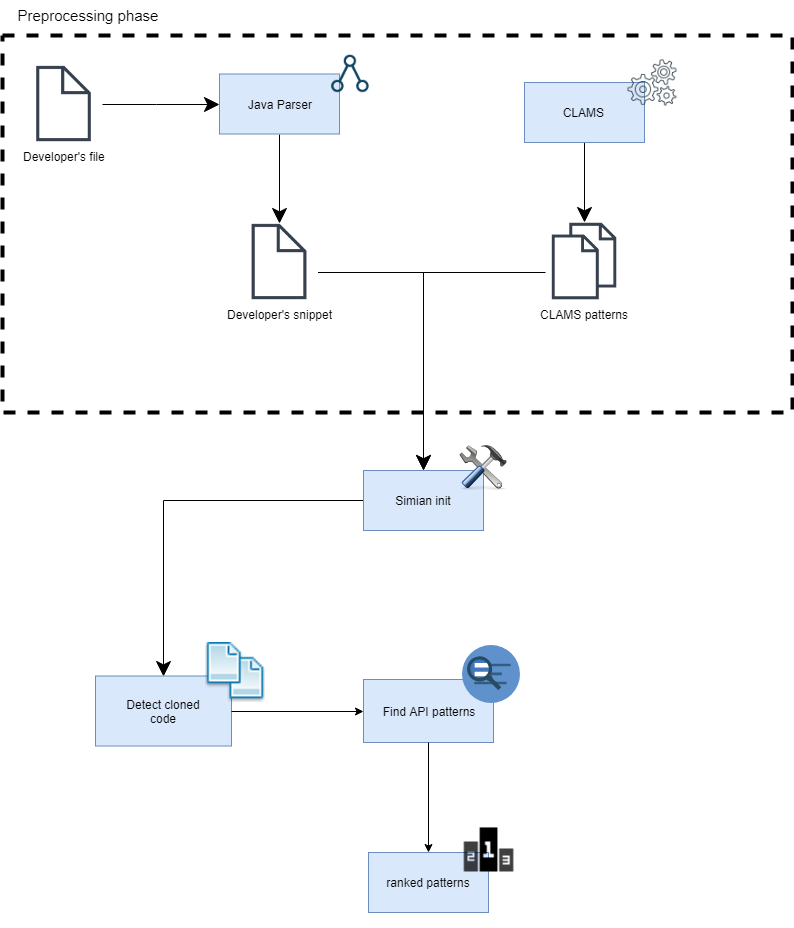
\includegraphics[width=14cm,height=16cm,keepaspectratio]{images/simian.png}
\centering
\caption{Overview of the proposed approach}
\label{fig:cmd}
\end{figure}

\subsection{Preprocessing}

About input files that are necessary to initialise the tool, we have from one side the developer's file with the real snippet of code that he is implementing and may want support for this. From the original file, we extract a portion that represent the context of the recommendation that can be a list of method invocations or simply a list of variable declaration. This portion is called ground truth and it is the part used as the context of the recommendation. On other hand, there are patterns mined by CLAMS, in form of ranked Java files sorted by rational specified in CLAMS paper. These file contains patterns, defined as sequence of API method calls that define, instantiate and using class belonging to the APIs contained in the developer' string. The number of these file and also their dimensions in term lines of code depend on the considered libraries. As Simian is a tool based on file comparison, we use temporary files of Java to do the comparison; after the process, the files are destroyed to reduce the amount of the space. \\
This preprocessing phase is required for Simian because, as we have seen in the related section, the tool not include any built-in preprocessing. To extract the snippet of code from the developer's file, we use Java parser,an open source project that allow to analyze, modify and generate Java code, to visit the AST of the input file and take the body of a method randomly selected that composes our ground truth. Notice that we consider only compilable files, otherwise Java Parser is not able to build the corresponding AST for the analysis. We take into consideration only the ground truth file because we are in the typical scenario in which the developer is starting to implement some features, so it writes only fragments of code, with a maximum length of 10 lines of code. Reversely, we don't consider an entire class or project, because in this scenario, the developer has completed almost the task and it is not interest in possible recommendations. 
As said before, in general a recommendation relies on the context in which the developer is implementing features. In our case, the context is the developer's code snippet with imports and variable declarations.\\
About CLAMS pattern, we create a golden set of 5 libraries, chosen among the 15 libraries provided by the authors on the website; for each of them, CLAMS retrieves a list of pattern represented by Java files and their number depends on the library that we consider. The precision and the lines of code of this list depends on the clients and examples files, as we described in CLAMS section when we talked about the existing approaches. We can also decide which methods and classes CLAMS analyze through the namespaces file in the proper folder. This phase is necessary because Simian doesn't have a well defined preprocessing phase and it is necessary to define in the proper way. We can define the entire procedure just described a human preprocessing, because we don't use any automatic procedure or heuristic algorithm to select the input files. Of course, we select relevant clients file, avoiding test classes, that are too smaller for our purpose and interfaces, that haven't no relevant body. For the CLAMS pattern, we don't put any limitation and we consider all possible patterns retrieved for a specific library.


\subsection{Simian within Eclipse platform}
Once we define the input, there is another step in order to use Simian to do API recommendations: the integration with Eclipse platform to have a more flexible and usable version of the tool, as Simian doesn't provide any IDE integration. As we said in related section, the basic version of Simian is a jar file launched from the terminal console with different options (see the Table 3). Although it is very easy to use, in this version is not very suitable for our purposes and it is necessary to integrate directly the Simian jar file, available on Simian website. To keep the integration with a Maven project, we create a repository that contain the update version of this jar and put it as reference in the POM file of the project. 
In order to integrate Simian in an Eclipse project, we have to set the following main classes: 

\begin{table}[H]

  \caption{ Overview about Simian classes }
  \label{Table:4}
\begin{adjustbox}{width=1\textwidth}

\begin{tabular}{|c|l|}

\hline
 \textbf{Simian class} & \textbf{Description} \\
\hline
 Auditstener & \vtop{\hbox{\strut This class is necessary to initialise Simian tool  } \hbox{\strut  and collect all notification from events that occur}} \\
\hline
Block & \vtop{\hbox{\strut This class represents the duplicated block of code as an object }\hbox{\strut and we can interact using method utilities}} \\
\hline
FileLoader &  \vtop{\hbox{\strut It is used to load all files}\hbox{\strut  for the comparison, with the method load}} \\
\hline
Checker &  \vtop{\hbox{\strut This class is used to perform the real comparison}\hbox{\strut  by calling the method check() on preloaded files}} \\
\hline
StreamLoader &  \vtop{\hbox{\strut Once we load files and create the Checker,}\hbox{\strut  this class load them into the Checker}} \\
\hline
Options &  \vtop{\hbox{\strut A data structure that encapsulates}\hbox{\strut  all options enabled for the comparison}} \\
\hline
Option &  \vtop{\hbox{\strut This class represents a single option}\hbox{\strut  and we can specify it by accessing to a static field}} \\
\hline
Language &  \vtop{\hbox{\strut This class contains static fields}\hbox{\strut  to set all supported languages as type of input files}} \\
\hline
CheckSummary &  \vtop{\hbox{\strut It contains all statistical data such as cloned code,}\hbox{\strut  number of total files, requested time and duplicated files }} \\
\hline
\end{tabular}

\end{adjustbox}
\end{table} 
The project has the following structure, divided in subpackages:
\begin{itemize}
\item business: it contains all the interfaces that expose the utility functions;
\item business.impl: It contains the classes that implement the interfaces and represent the business logic of the entire application;
\item model: It contains the representation of the SimianPattern object, useful to keep all information for the cloning phase;
\item evaluation: It contains all the functions necessary for the evaluation framework, specified in the proper section.
\end{itemize}
Going in deep on the business implementation, we have three main classes: SimianDataExchangeImpl, that performs the code cloning activity and collects all data needed for the analysis, APICallRecommederImpl, that takes the data from Aulistener and filter them and SimianFileUtilitiesImpl, that contains all the operation related to files. In particular, SimianDataExchangeImpl implements the original Simian class showed in the table above and it initialize the tool in order to perform the code cloning activities. Among the implemented methods, we use the function \textit{block()} retrieve all necessary information for a duplicated block of code and the file that contains it. The \textit{endCheck()} function is called at the end of the process and manipulated the class CheckSummary mentioned before. In this way, we can obtain all information the total number of analyzed files, the duplicated ones, the time required for the comparison and the total number of blocks. This class implements also the ExchangeData interface, that is used as a bridge for ApiCallRecommenderImpl class, as Simian interface provide only void methods without the possibility to return the necessary information.\\
Going further, we describe now the APICallRecommenderImpl class, that collects the data coming from the previous class and analyze them in order to produce the recommendation. The main function is \textit{findPattern()}, that loads the necessary files and launch Simian analysis exploiting the Aulistener interface. The files are loaded in pairs, in which we have the snippet of code coming from the developer's file and the other component is the list of CLAMS pattern. During the analysis phase, it is necessary to check the files and in particular, we have to discard from the analysis the files that contains duplicated blocks within themselves. It is possible because Simian retrieve for each pairs the files that contains a duplicated blocks of code and, in this way, we can reduce some bias lead to the fact that in the developer's snippet we can have some duplicated lines of code that are not interesting for the recommendation. Once we have the block, we can create the object SimianPattern that represent the discovered pattern for the snippet among the CLAMS results.\\
The class for this object belongs to the model subpackage, that represent the extracted pattern. Following the POJO structure, we have getter and setter functions for each property of the object, gradually filled during the analysis. We have duplicated lines to store the cloned code, the filename of the pattern and the elapsed time for each pattern that Simian has found in the analysis. In this way, we can easily write in a file to show the final results in a more understandable way. The original Simian output, in facts, shows only the duplicated lines and CLAMS puts the patterns in a ranked list but without the context, represented in this case by the import at the beginning of the file. Thanks to this structure, we can also rank the patterns from the one that have more lines in commons, using the proper field in the wrapper class.\\
The last main component is SimianFileUtilities, in which we open all necessary files, write the recommendations and create temporary files for the code cloning activity. All these classes are integrated in test class that calls in the proper sequence all the methods to perform the final recommendation. In particular, the method \textit{scan()} takes all files that contains patterns extracted by CLAMS while the function \textit{createTemporaryFile()} creates the temporary files to perform the comparison. To extract the ground truth part used in the evaluation part, we use the function \textit{parseAST()}. This function uses JavaParser library to visit the AST and takes the body of the method that we are interested in. In this way, Simian inputs are only partial fragments of code that represent the typical developing scenario. \\
The project contains also classes with the evaluation task, such as the function to build the Rascal project structure in order to analyze the corresponding method invocations and to apply the metrics on them. More details on it is provide in the evaluation framework section. 
The overall architecture is depicted in Figure 5, in which components represent the described features.
\begin{figure}[H]
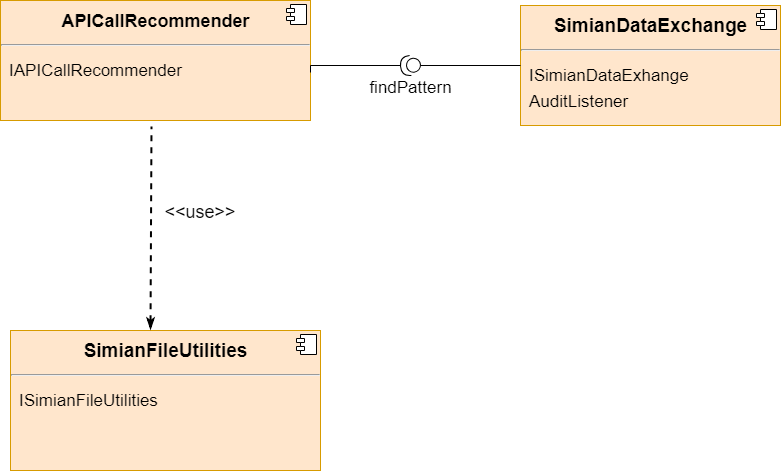
\includegraphics[width=12cm,height=12cm,keepaspectratio]{images/Component.png}
\centering
\caption{Component diagram}
\label{fig:cmd}
\end{figure}

\subsection{CLAMS adaptation}
Regarding the CLAMS output, we describe the original structure as well as the necessary modification to integrate it in our approach. The authors, differently from other works, provide the complete source code and commands to set up the entire environment to have CLAMS working on Linux . CLAMS is written in Python and uses srcXML and Astyle to produce XML files and to formatter in a human-readable way the code respectively, but as claimed by the authors, there is no really constrain about the technologies to use in case of a new implementation. As input, CLAMS takes two kind of files: client files, that represent the real project on Github related to the dataset that authors use for evaluation phase while example files are used as training set.\\ 
All these files are collected in a folder, that CLAMS loads by getting the path. Moreover, there is a namespace file that identify the name of classes used in the clients and example files by using their complete namespaces such as org.codehaus.jackson. The last input used by the main.py file, that is used to initialise the platform, is the list of methods that are represented by an ARFF(Attribute-Relation File Format) file~\cite{https://www.cs.waikato.ac.nz_last_nodate}, used in the machine learning domain. It is an ASCII text file that describes a list of instances sharing a set of attributes, specified in the header section. In our case, the attributes are the method declaration (the caller) and the method invocations (the calls). 
If we want to add some other libraries with respect to the original dataset (MQTT-Json projects), we need to replicate the same structure for CLAMS; to do this, we found on Github several projects related to this libraries and produce the ARFF files using Rascal, as we will see in the validation section
\newline
There is a phase of preprocessing in which CLAMS extracts API call and their AST using JDT utilities and represent them in xml using srcXML. The core of the project is the snippet generator module (represented by summarise.py file) that takes as input a source code file (java in this case) and using srcXML they first replace literals with xml types and delete comment. Then, they separate the API code from code that doesn't contain API call and highlights the variable in local scope of API. Finally, the code without API call is removed and Clams add some comments near the API statement and needed variables. Notice that their approach considers also the classical statement like if-else structure as a part of API statement. \\
For clustering, they use both HDBSCAN and k-medoids algorithm that are quite similar and differs only in the precision of the returned snipped (HDBSCAN is more accurate but k-medoids covers more methods). For both of them, the authors import Python libraries that implement these algorithm quite well and we can switch the algorithm by change the parameter in the main.py. Moreover, they have the file ranking.py to order the generated snippet. The rank is based on the example files that contains a sequence of API call; if the sequence within the file is a super-sequence of the sequence of snippet that we considered, so this snippet is supported, and its rank is increased. In the result folder, CLAMS put the library that we want to analyze, the methods, the source file (both in .java and xml format), some JSON file that represent all information about a method (class, package, rank, id) and the arff file related to the library. \newline
For the integration step in our platform, it is necessary to slightly modify the original approach to have better results. In particular, if we use the pattern of CLAMS as they are, there are some bias because, through srcML, CLAMS substitutes the literals with its own type and Simian is not able to detect them as cloned code, even using all available options regarding the code. So, to avoid this situation, we must modify the function that substitute literals, putting some default value instead of srcML types. This modification doesn't affect the validity and accuracy of extracted path because is just a matter of modify literals with another and allow Simian to avoid bias in the code cloning analysis.

\subsection{API recommendations}
At the end of these preparatory phases, we describe now the core of this project, the API recommendations. Once the Simian is launched as we described, it performs the detection of code cloning activity on the CLAMS patterns files and the developer's code snippet. The typical scenario is depicted by the use case diagram in Figure 6, in which the developer asks for recommendations.


\begin{figure}[H]
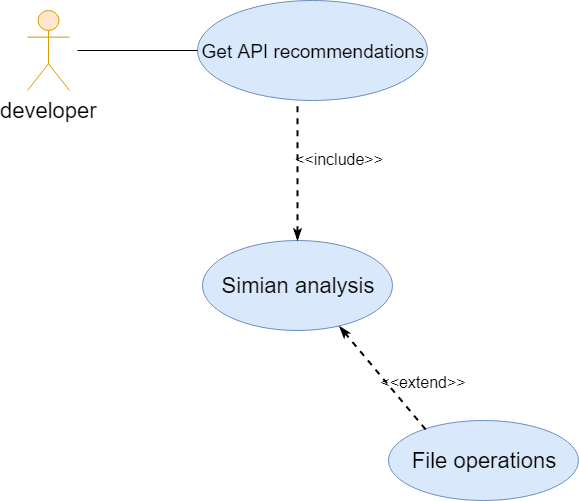
\includegraphics[width=10cm,height=10cm,keepaspectratio]{images/Usecase.png}
\centering
\caption{Use case scenario}
\label{fig:cmd}
\end{figure}

Notice that the notion of cloned code depends on the options that we have selected and turn on: the mandatory options to enable is the threshold, that set the minimum line of code in commons, reportDuplicateText, otherwise we couldn't show and manipulate the result and language that is Java because we analyze projects related to it. Without this options, Simian gives us only the fingerprints that represent the source coordinates of the files, that are not significant for our aims. So, to have a better representation, we have put the results in a wrapper class that represent the Pattern object in which we have all attributes to describe in the right manner the recommendation.\\
Other options, such as the strings, identifiers or modifiers that should be introduced in the comparison, can be enable with respect to the level of cloning that we want to reach. To find useful results, it is necessary to set at least ignoreIdentifiers, ignoreIdentifierCase, ignoreLiterals, ignoreVariableName, ignoreNumbers and ignoreModifiers because, in this way, Simian goes beyond the developer personal implementations and looking only for the structure of the code, in order to use the concept of pattern in a more effective way. Based on these options, Simian applies the proper transformations on the original textual code in order to perform the comparison. 
Furthermore, Simian compares the pair developer' snippet - pattern because some CLAMS pattern includes some duplicated lines of code and this can bring some bias. Once we load the files, the check is performed and the results that include lines of code, name of pattern file and time to perform the comparison and put all in the wrapper class mentioned before.\\
At the end of this step, we have the patterns (a complete one or only partial) that the developer is start to implement and we can discard it from the comparison, as the developer is not interested to see what he have done so far. The last step is remove the duplicated line of code from the suggested pattern and show to the developer only the novel part, that integrate his code or propose new pattern for that feature, related of course to the library that he is implementing. About the ranking, we order the pattern by considering the number of cloned lines, so the first pattern is the contains more duplicated lines rather than second and so on. The rank phase is simply performed on the SimianPattern object that we produce as output. All the steps are summarized in the Sequence Diagram below.

\begin{figure}[H]
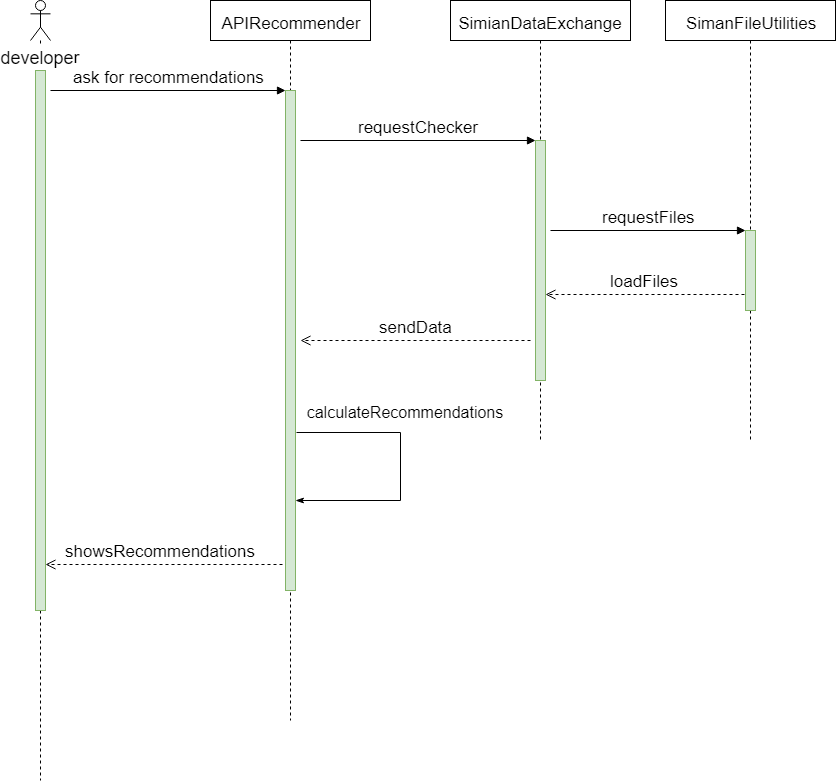
\includegraphics[width=14cm,height=16cm,keepaspectratio]{images/Sequence.png}
\centering
\caption{Sequence diagram }
\label{fig:cmd}
\end{figure}


In the example below, related to MQTT paho library, we have extracted the method publish() from the developer's file with Java Parser and run Simian on it.  The last columns shows two top rank CLAMS patterns related to it.
\vspace{5mm}

Developer's original file
\begin{lstlisting}
package org.eclipse.paho.sample.mqttv3app;
import java.io.IOException;
import java.sql.Timestamp;
import org.eclipse.paho.client.mqttv3.IMqttDeliveryToken;
import org.eclipse.paho.client.mqttv3.MqttCallback;
import org.eclipse.paho.client.mqttv3.MqttClient;
import org.eclipse.paho.client.mqttv3.MqttConnectOptions;
import org.eclipse.paho.client.mqttv3.MqttException;
import org.eclipse.paho.client.mqttv3.MqttMessage;
import org.eclipse.paho.client.mqttv3.persist.MqttDefaultFilePersistence;

public class Sample implements MqttCallback {		
   	public Sample(String brokerUrl, String clientId, boolean cleanSession, boolean quietMode, String userName, String password) throws MqttException {    	
    		try {    		
	    	conOpt = new MqttConnectOptions();
	    	conOpt.setCleanSession(clean);
	    		if(password != null ) {
	    	  		conOpt.setPassword(this.password.toCharArray());
	    		}
	    		if(userName != null) {
	    	  		conOpt.setUserName(this.userName);	   
	    		}    		
			client = new MqttClient(this.brokerUrl,clientId, dataStore);		
	    	client.setCallback(this);
	    	
		} catch (MqttException e) {
			e.printStackTrace();
			log("Unable to set up client: "+e.toString());
			System.exit(1);
		}
    }

    public void publish(String topicName, int qos, byte[] payload) throws MqttException {
    	
    	// Connect to the MQTT server
    	log("Connecting to "+brokerUrl + " with client ID "+client.getClientId());
    	client.connect(conOpt);
    	log("Connected");   	
    	String time = new Timestamp(System.currentTimeMillis()).toString();
    	log("Publishing at: "+time+ " to topic \""+topicName+"\" qos "+qos);    
   	MqttMessage message = new MqttMessage(payload);
    	message.setQos(qos);     
    	client.publish(topicName, message);    	
    	// Disconnect the client
    	client.disconnect();
    	log("Disconnected");
    }
    
  
    public void subscribe(String topicName, int qos) throws MqttException {    	    
    	client.connect(conOpt);
    	log("Connected to "+brokerUrl+" with client ID "+client.getClientId());    
    	log("Subscribing to topic \""+topicName+"\" qos "+qos);
    	client.subscribe(topicName, qos);
    	// Continue waiting for messages until the Enter is pressed
    	log("Press <Enter> to exit");
		try {
			System.in.read();
		} catch (IOException e) {
			//If we can't read we'll just exit
		}		
		// Disconnect the client from the server
		client.disconnect();
		log("Disconnected");
    }
}
\end{lstlisting}


\vspace{5mm}
\newpage
Extracted method:
\begin{lstlisting}

   // Connect to the MQTT server
    log("Connecting to " + brokerUrl + " with client ID " + client.getClientId());
    client.connect(conOpt);
    log("Connected");
    String time = new Timestamp(System.currentTimeMillis()).toString();
    log("Publishing at: " + time + " to topic \"" + topicName + "\" qos " + qos);
    // Create and configure a message
    MqttMessage message = new MqttMessage(payload);
    message.setQos(qos);
    // Send the message to the server, control is not returned until
    // it has been delivered to the server meeting the specified
    // quality of service.
    client.publish(topicName, message);
    // Disconnect the client
    client.disconnect();
    log("Disconnected");
 \end{lstlisting}
\vspace{5mm}

\begin{minipage}[t]{0.5\textwidth}
\begin{lstlisting}
CLAMS pattern #1

{
    String pubTopic;
    MqttClient pubClinet;
    String payload;
    int qos;
    pubClinet = new MqttClient(url, clientId);
    pubClinet.setCallback(this);
    pubClinet.connect();
    MqttMessage message = new MqttMessage(payload.getBytes());
    pubClinet.publish(pubTopic, message);
    pubClinet.disconnect();
}
\end{lstlisting}
\end{minipage}
\begin{minipage}[t]{0.5\textwidth}

\begin{lstlisting}
CLAMS pattern #2

{
    String topicName;
    MqttAsyncClient client;
    MqttConnectOptions conOpt;
    String brokerUrl;
    byte[] payload;
    int qos;
    log("a string"+brokerUrl + "a string"+client.getClientId());
    IMqttToken conToken = client.connect(conOpt,null,null);
    log("a string"+System.currentTimeMillis()+ "a string"+topicName+"a string"+qos);
    IMqttDeliveryToken pubToken = client.publish(topicName, message, null, null);
    pubToken.waitForCompletion();
    IMqttToken discToken = client.disconnect(null, null);
    discToken.waitForCompletion();
}

	
\end{lstlisting}
\end{minipage}
\newline
In particular, the two extracted recommendations show two possible use of the object MqttMessage that the developer declare in the publish method. The first recommendation add an MqttClient while the second use the interface IMqttDeliveryToken as a different way to send the mqtt message. Of course, the number of recommendation is strongly related to the length of the method and how many lines Simian can detect in its textual analysis. This example is just to show the expected output after running our approach. In general, given a project that uses different libraries, with this approach we are able to recommend patterns of whatever libraries that the user are interested to develop. As mentioned before, recommendations are at level of code snippet, that provide a concrete and immediate hint. As we choose CLAMS for the second element of the clone pair, we are not able to provide tutorial or complete application as recommendation, because only the patterns are available for this purpose. \\
We can support almost the dataset of CLAMS, because the authors provides all necessary files on Github to have the patterns, but we can support also different libraries like MQTT or Json. Notice that quality of recommendations depends first of all on the blocks in the developer's file that Simian is able to detect in the patterns provided by CLAMS. More patterns means more support for the library and this bring more API recommendations at the end of the process. An other aspect to taking into account is that Simian analyse the duplicated blocks of code and maybe some methods invocations that are not in the correct sequence are discarded automatically from the final recommendation. \\
In next section we set up an evaluation framework  by using part of the dataset of CLAMS (as we have already the patterns used by Simian for the comparison). We do this as a double check validation because Simian not have a postprocessing phase as we said in the related section and we need a comparison that goes beyond the lexical one in order to apply the metrics. Moreover, we will compare the Simian results with PAM, already described in the existing approach section.





	
	
	\chapter{Evaluation}
	\label{sec:threats}
	At this point, we proceed with the evaluation of the results showed in the previous section. As the concept of recommendation changes from a context to another and it depends also on the developer's skills (maybe a more expert user finds a certain recommendation less useful rather than a not expert user), we look for an evaluation framework that evaluates the results without bias related to this aspect. To do this, we choose Rascal tool to parse the AST of the developer's file and the API recommendations obtained combining Simian and CLAMS results. From Rascal, we obtain a list of method declarations and the related invocations for each file and compare them in order to calculate four metrics: precision, recall, success rate and F measure. These metrics are very useful because they allow to analyze the results at more abstract level, going beyond the code cloning activity. In facts, as we said in the related section, Simian not perform this kind of comparison because it is a textual code cloner and looks only for duplicated lines of code. The main structure of the validation framework is depicted in Figure 9. Moreover, we compare the proposed approach with PAM, the probabilistic tool already analyzed in term of results, computational time and also by applying the same metrics on the method invocations. Next sections explains in details each component of this system, especially how to run Rascal and how the metrics have been calculated and how covert the PAM format in order to perform the comparison in the right manner.




\begin{figure}[!h]
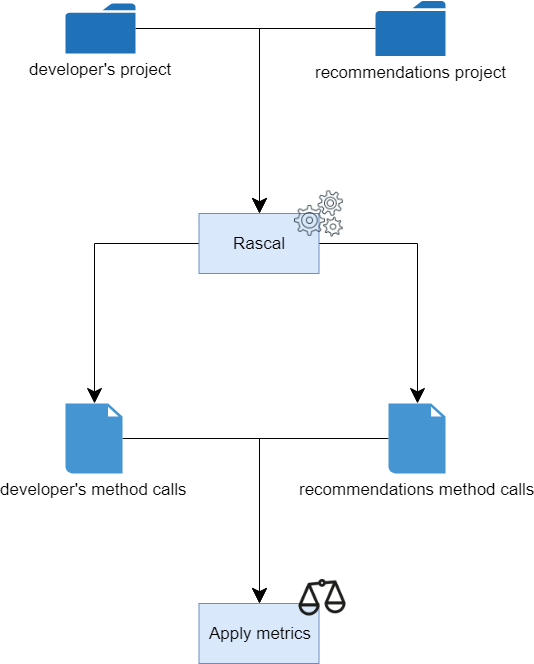
\includegraphics[width=14cm,height=14cm,keepaspectratio]{images/rascal.png}
\centering
 \caption{Validation framework}
 \label{fig:cmd}
\end{figure}

\section{Research questions}
The research question are the following: \\

\textbf{RQ$_1$} \textit{ Is it the approach able to provide consistent recommendation?}
This research question measures the quality of the recommendations provided by comparing the context, represented by the round truth part, and the retrieved patterns by the proposed approach. We analyze possible situation in which there are some false positive situations by computing the metrics mentioned before and report the results in order to make an evaluation at the level of method invocations.\\
\textbf{RQ$_2$} \textit{Are the final results good enough compared with PAM?} In order to validate the proposed approach, we perform a comparison with PAM, the tool presented in the existing approach section and compute the metrics also on it. We provide a comparison between the two approaches by looking the average metrics values. PAM produces a list of method invocations, so to do in a better way the comparison we used Rascal to transform the recommendations provided by our approach in method invocations. It is necessary to computes the metrics\\

\textbf{RQ$_3$} \textit{What are the timing performances of the proposed approach?} With this research question, we measure the time computation for a single recommendation. We take into account also the time needed to write the output file with the recommended snippet of code and compare it with PAM. We added the time comparison because it is crucial factor in a recommendation system. We measure the time in seconds.\\

\section{Study methodologies}
To validate and apply the metrics, we simulate the typical scenario in which the developer is working on a project. To do this, we select randomly a fragment of code coming from the client file using Java Parser as described before. We obtain in this way our context, that is only a small part of the original file and perform our approach on it. To apply metrics, however, we need a transformation from the snippet of code to method invocations, that is a more comparable format. To do this, we use Rascal~\cite{utor.rascal-mpl.org/_last_nodate}, a language for meta programming and it is able to create programs that read, analyse, transform, generate and/or visualize other programs. The range of programs to which meta-programming can be applied is large: from programs in standard languages like C and Java to domain-specific languages for describing high-level system models or applications in specialized area. In some cases, even test results or performance data are used as input for meta-programs. \\
We look also to the kinds of meta programs that can be analyzed by Rascal like reverse engineer and statically analyse of a big software system before visualizing the results. The principal aim of Rascal is to provide a reusable set of primitives to build and manipulate program representations. The point is not to be or provide a unified representation of programs to let generic algorithms operate on.  
We can look also at Rascal as an engineering tool for programmers that need to construct meta programs because it allows running, inspecting, debugging, tracing, profiling, etc. just as normal programs do. The main advantages are:
\begin{itemize}
\item The syntax is very easy to learn and is used even for model and represent sophisticated concepts;
\item Sophisticated built-in data types provide standard solutions for many meta-programming problems;
\item Safety is achieved by finding most errors before the program is executed, so the debug phase is reduced;
\item Local type inference makes local variable declarations redundant;
\item Pattern matching can be used to analyze all complex data structures;
\item Syntax definitions make it possible to define new and existing languages for specific purposes;
\item Traversing the data structures is doing in an effective way and it is possible to extract information from them or to synthesize results;
\item Templates enable easy code generation;
\item The integration in Eclipse simplify the usage and the iteration with all Rascal features.
\end{itemize}
Moreover, Rascal implements the so called EASY(Extract-Analyze-SYnthesize) paradigm, used in the meta programming domain. Any meta-programming problems follow a fixed pattern. Starting with some input system (a black box that we usually call system-of-interest), first relevant information is extracted from it and stored in an internal representation. This internal representation is then analyzed and used to synthesize results. If the synthesis indicates this, these steps can be repeated over and over again. The figure below represents the EASY paradigm that is quite common in the meta programming domain.

\begin{figure}[!h]
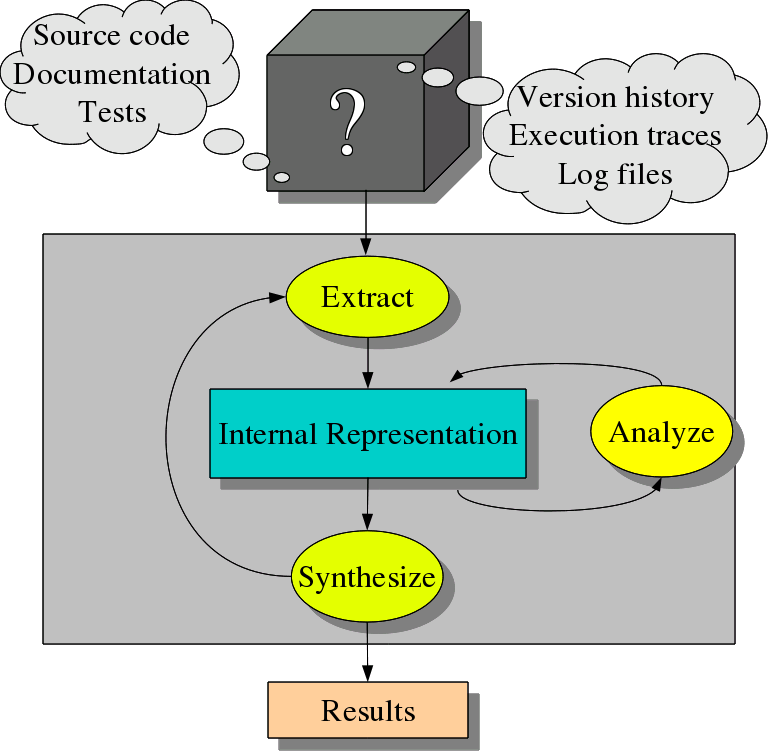
\includegraphics[width=10cm,height=12cm,keepaspectratio]{images/EASY.png}
\centering
  \caption{The EASY paradigm used by Rascal}
  \label{fig:cmd}
\end{figure}

For our purposes, we use Rascal to parse AST of an entire project and retrieves all necessary information from it, such as class names, packages, methods and variables.
To do this, however, it needs a runnable project and the classpath file in which all dependencies are specified. In our scenario, the only required dependency is the jar file for the library. As the evaluation takes places among method invocations, we are forced to create this structure for the developer's file and the patterns that represents our recommendations. The structure is represented in Figure 11, in which we have:
\begin{itemize}
\item src folder: it contains the Java file with the source code;
\item lib folder: it contains the jar files that represent the libraries used in the project;
\item classpath file: it contains the dependencies for the project.
\end{itemize}

\begin{figure}[!h]
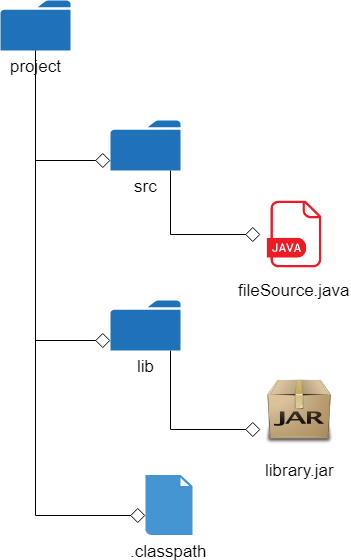
\includegraphics[width=12cm,height=12cm,keepaspectratio]{images/Folders.png}
\centering
  \caption{Folder structure for Rascal}
  \label{fig:cmd}
\end{figure}

Where the file in the src folder represents the developer's file in one project and the recommendations in the second one. These two projects will be the input of Rascal. All the structure is built in the evaluation subpackage as mentioned before. In particular, we functions that takes as input the library name and gives the correct classpath file to have the structure mentioned before. Moreover, we have a function that build the class in the correct way putting together the CLAMS patterns in a single class (for each of them, the function creates a method) where at the beginning the same import of the ground truth are inserted. For the patterns, we take as import the same contained in the namespaces file included in the original CLAMS dataset, in order to have all possible method invocations. \\
Also for the ground truth we make a similar structure, by putting the considered method in a Java class in the Rascal structure. We make this task for the ten client projects for each considered library twice, because we want to analyze also the pattern in form of snippet of code extracted by the proposed approach. For the ground truth fragments of code, we put all imports used in the original client file; for the mined patterns, we encode in the built files all the imports that belong to the CLAMS namespace file. This task is necessary because we don't know at the beginning what are all the possible recommendations and so the possible method invocations. This approach cannot bring any bias because Rascal retrieves only the method invocations with the corresponding import. Here below we have an example file created for Rascal:
\newpage
\begin{lstlisting}
import twitter4j.Query;
import twitter4j.Tweet;
import twitter4j.Twitter;
import twitter4j.TwitterFactory;
public class Twitter4jSample{
public void ground() {
    List<MyTweet> tweets = new ArrayList<MyTweet>();
    try {
        // get some tweets about java
        Twitter twitter4j = new TwitterFactory().getInstance();
        for (int i = 0; i < 3; i++) {
            Query q = new Query("java");
            q.setRpp(100);
            for (Tweet tw : twitter4j.search(q).getTweets()) {
                MyTweet myTw = new MyTweet(tw.getId(), tw.getFromUser());
                myTw.setText(tw.getText());
                myTw.setCreatedAt(tw.getCreatedAt());
                myTw.setFromUserId(tw.getFromUserId());
                tweets.add(myTw);
            }
            Thread.sleep(1000);
        }
    } catch (Exception ex) {
        logger.error("Error while grabbing tweets from twitter!", ex);
    }
    return tweets;
}
}
\end{lstlisting}
In particular, we have added the fragment of code pick up from the developer's client file and put it a method called ground, plus the required imports for the snippet.
Once we setup this structure in this way, Rascal is able to parse the AST and retrieve the list of method invocations used to validate the approach.
Rascal is launched using Eclipse RCP-RAP as platform and, for this reason, we must use it as standalone to produce the list of method invocations starting from the output file of Simian and CLAMS. The main component of Rascal is module in which we define the function used for our purpose. In particular, the proper function is called on the project's folder and gives as output a file that contains the method invocations. As we said, it is possible by creating the AST and takes from it method declaration and invocations. Here below, we can see an example of a set of method invocations, related to the previous MQTT ground truth example and the second one that contains the method invocations of the mined patterns by Simian related to the MQTT library:\\
Method invocations of the ground truth

\begin{lstlisting}
MqttSample/ground()#org/eclipse/paho/client/mqttv3/MqttMessage/MqttMessage(byte[])
MqttSample/ground()#org/eclipse/paho/client/mqttv3/MqttMessage/setQos(int)
MqttSample/ground()#java/lang/System/currentTimeMillis()
\end{lstlisting}

\vspace{5mm}
\noindent
Method invocation of the mined patterns
\begin{lstlisting}
MqttSample/pattern56()#org/eclipse/paho/client/mqttv3/MqttMessage/MqttMessage(byte[])
MqttSample/pattern56()#org/eclipse/paho/client/mqttv3/MqttClient/MqttClient
(java.lang.String,java.lang.String)
MqttSample/pattern56()#org/eclipse/paho/client/mqttv3/MqttClient/disconnect()
MqttSample/pattern56()#org/eclipse/paho/client/mqttv3/MqttMessage/setQos(int)
MqttSample/pattern56()#org/eclipse/paho/client/mqttv3/MqttClient/publish
(java.lang.String,org.eclipse.paho.client.mqttv3.MqttMessage)
MqttSample/pattern56()#org/eclipse/paho/client/mqttv3/MqttClient/connect()
MqttSample/pattern56()#java/lang/String/getBytes()
MqttSample/pattern56()#org/eclipse/paho/client/mqttv3/MqttClient/setCallback
(org.eclipse.paho.client.mqttv3.MqttCallback)
MqttSample/pattern59()#org/eclipse/paho/client/mqttv3/MqttMessage/MqttMessage(byte[])
MqttSample/pattern59()#org/eclipse/paho/client/mqttv3/MqttMessage/setQos(int)
MqttSample/pattern59()#org/eclipse/paho/client/mqttv3/IMqttToken/waitForCompletion()
MqttSample/pattern59()#java/lang/System/currentTimeMillis()
MqttSample/pattern27()#org/eclipse/paho/client/mqttv3/MqttMessage/MqttMessage(byte[])
MqttSample/pattern27()#org/eclipse/paho/client/mqttv3/MqttMessage/setQos(int)
MqttSample/pattern27()#org/eclipse/paho/client/mqttv3/MqttMessage/setRetained(boolean)

\end{lstlisting}
As it is, these files are not so suitable for an immediate analysis. However, we can apply metrics used in the statistic and information retrieval domains in order to evaluate the Simian approach going beyond the lexical code cloning activity, trying to evaluate the results from a different point of view.
We also select the code fragments that compose our ground truth, trying to coverage the most important objects and methods for each library. To do this, we compose different scenarios, one in which Simian analyzes the first lines of a certain method, another in which we pick the last method and so on. The aim is to cover all the possible features that a certain library offers. For example, for Twitter4j library, we select snippets of code that have both methods for user authentication procedure and methods and procedure to publish a tweet.
\section{Dataset}
First of all, we show the list of libraries that the proposed approach supports. They are the same of CLAMS, as they are already tested and most popular in the Java project context. We select 5 libraries among the CLAMS original dataset and they are showed in Table 7. In the table we show also the number of recommended pattern provided by CLAMS, that measure the level of support offered by it. For each library, we select 10 files among these files in order to keep the same context and to perform average values for the metrics. From this, we build our dataset that contains 50 files. Notice that each file represent the developer's file that we have seen in the proposed approach figure and we extract from them the ground truth part. For each of them, we run the proposed approach and evaluate the results through the metrics and the comparison with PAM.
\begin{table}[!h]
  \caption{ Libraries supported by Simian and CLAMS }
  \label{Table:7}
 \begin{center}

\begin{tabular}{|c|c|c|}

\hline
 \textbf{Library} & \textbf{No. of patterns}  \\
\hline
 twitter4j &  107   \\
\hline
drools & 309 \\
\hline
camel & 152  \\
\hline 
wicket & 717  \\
\hline
restlet-framework & 182  \\
\hline
\end{tabular}
\end{center}
\end{table} 
Here we provide also a brief description of the our golden set:
\begin{itemize}
\item twitter4j: it is used for integrate the Twitter services in Java environment;
\item drools: it is a Business Rules Management System(BRMS) that helps to define the internal rule for the language;
\item camel: it defines mediation rules and routing for specific domain languages;
\item wicket: it is a component based web framework;
\item restlet framework: it helps to build web APIs following the REST architecture. 
\end{itemize}




\section{Metrics}
Once we have the two lists of method invocations, we can define metrics to do the evaluation. They are precision, recall,  f measure and success rate showed below:\\


\begingroup

\fontsize{15pt}{24pt}\selectfont
\noindent
$ Precision =  \frac{corr}{all_{rec}}\\  
\\
Recall  = \frac{corr}{all_{gt}} \\  
\\
F\,Measure =\frac{2*precision*recall}{recall+precision}\\
$

\begin{equation}
 \text{Success rate} =
    \begin{cases}
      1 & \text{if at least one method of the ground truth }\\
      & \text{belongs to the recommended pattern invocation}\\      
      0 & \text{otherwise}
    \end{cases}       
\end{equation}

\endgroup



Where the $corr$ is the number of correct API method invocations by the approach related to the context, $all_{rec}$ is the number of method invocations in the recommendations and $all_{gt}$ are all method invocations of the ground truth part, extracted from the initial files. With the first metric, we want to measure the precision of the recommendations related to the context considering all the patterns and so all the method invocations related to them. The recall, instead, point out the rate related to the ground truth part, that is more restricted than the original file and so, in this case, Simian gives as out put less method invocations but more focused on the context in which we are. The F measure considers both precision and recall in order to give an average value on the accuracy of the approach. The classical index considers the harmonic mean between precision and recall. Finally, the success rate is a binary value that is equal to 1 if at least one method in the ground truth is found in the recommendation, 0 otherwise. In the table, we measure this index for all ten clients and so we give a rate that represents an average success rate.\\
All the rates goes from 0 to 1 and represent the accuracy of the approach. These number is affected also by the number of patterns extracted by CLAMS. The metrics are computed by using Eclipse, and in particular, once we have the files coming from the Rascal computation, described in the previous section, the function applyMetrics calculates all the metrics specified above.

\section{Results}

These metrics work on the method declarations and invocations, so for each mined patterns by the approach we can have a taste of the results. In particular, we go further with respect to the code cloning analysis, that looking for only the lexical differences among the lines of code. Reversely, we are able to adding some postprocessing phase on the results and we can do more accurate comparison with this evaluation framework. 
We also make a comparison between the proposed approach and an existing API recommendations already presented in the related work section, PAM. The metrics are useful to evaluate the accuracy of Simian applied to CLAMS but we decide to improve the validation framework adding an existing and validated approach. As we said, PAM uses probabilistic techniques in order to retrieve the most probable method invocation starting from file in ARFF format, that contains method invocations and declarations. We can compare the result of PAM with the proposed approach considering the top rank method invocations retrieved by CLAMS (notice that the ranking is based on the duplicated lines of code founded between the original code and the patterns). As the format of our recommendation strongly differs from the PAM format, we have to used once again Rascal to extract the method invocations that represent the API recommendations of the ground truth. What is different is the ranking method to order the list of method invocations. The real issue is to bring the code snippet format towards the PAM format to make a fair comparison.\\
To do this, first of all we have to the same inputs for the tools involved in the comparison. In the case of CLAMS, we can keep trace of the context with the ARFF, that contains the method caller and calls for the library as we described in the proper section, and the clients file, that represent the real implementation in Java. On the other hand, PAM takes as input only the ARFF file without any clients files for the context; so, it is necessary to represent the context in we are in order to reduce bias in the analysis. We can do this by converting the clients files (that are Java source code) in the ARFF format and combine the original files with this new one. We can reuse Rascal in the same way seen in the metrics evaluation, by extracting the method invocation from the clients file. After this phase, we have to transform the method invocations into ARFF format. We can do this with a Python script that converts the file in the right format and combine the original ARFF file with the clients invocations in only one file, that represent the developer's context. In this way, PAM is able to keep trace of the context and produce as final output the list of API function call. After we run PAM, it produces the results in the format already specified in the proper section, in form of method invocations and the corresponding probability. However, as the ground truth are usually only a fragment of the original developer's file, the invocations have small probabilistic impact because the original ARFF file for each libraries have more than 2,000 lines. So, in order to apply metrics for the comparison, we are forced to split the PAM result files and select the section in which we find proper invocations. The figure explains all phases needed for obtain the same format used in the comparison:
 

\begin{figure}[!h]
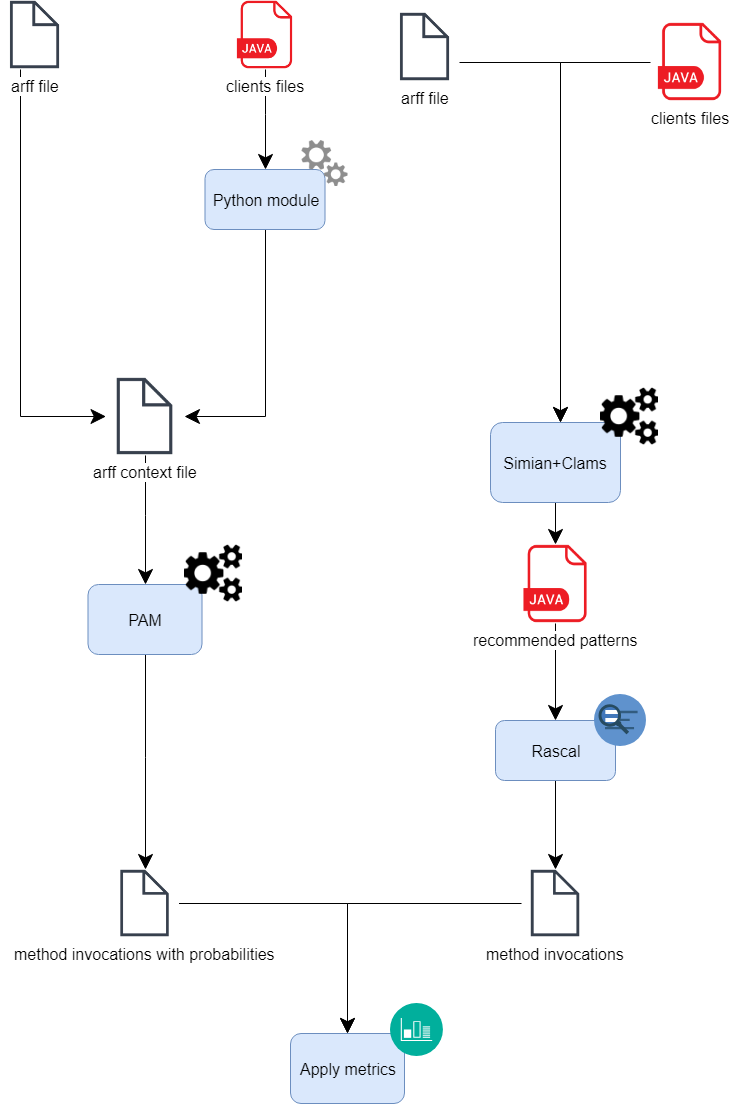
\includegraphics[width=18cm,height=18cm,keepaspectratio]{images/PAM.png}
\centering
  \caption{Process for PAM comparison}
  \label{fig:cmd}
\end{figure}
 At the end of the process, we have the list of invocations ranked by probabilities from PAM and the list of invocations extracted by Rascal. As we have the same format, we can apply the metrics in the same way described before. The two tables offers a comparison between the proposed approach and PAM: 

\begin{table}[!h]
  \caption{ Average values for the proposed approach }
  \label{Table:8}
 \begin{center}
\begin{tabular}{|c|c|c|c|c|}

\hline
 \textbf{Library} & \textbf{precision}  & \textbf{recall} & \textbf{success rate} & \textbf{F-measure} \\ 
\hline
 twitter4j &  0,506235119 & 0,74285538 &  0,9 & 0,545789625 \\
\hline
drools & 0,22455129 &   0,344444445 & 0,7 & 0,215914793\\
\hline
camel & 0,430785693  & 0,598096273 & 1 & 0,448844577 \\
\hline 
wicket & 0,104704642 & 0,23564139 & 0,6 & 0,152584271 \\
\hline
restlet-framework &  0,292169883 &  0,539874547 & 0,7 & 0,218620598  \\
\hline
\end{tabular}
\end{center}
\end{table} 

 
 \begin{table}[!h]
  \caption{ Average values for PAM}
  \label{Table:4}
 \begin{center}
\begin{tabular}{|c|c|c|c|c|}
\hline
 \textbf{Library} & \textbf{precision}  & \textbf{recall} & \textbf{success rate} & \textbf{F-measure} \\ 
\hline
 twitter4j & 0,471779376  & 0,601220656 & 0,9  & 0,443219823  \\
\hline
drools & 0,224551356 & 0,467142966   & 0,7 & 0,261774121 \\
\hline
camel & 0,243655335  & 0,562697394 & 0,7 & 0,238838121 \\
\hline 
wicket &0,080743729  & 0,358903284 &  0,6 & 0,119715519  \\
\hline
restlet-framework & 0,246895116  & 0,377042229 & 0,7 & 0,235095648 \\
\hline
\end{tabular}
\end{center}
\end{table} 
This results are useful to answer the questions \textbf{RQ$_1$} and \textbf{RQ$_2$}. We can see the results of the proposed approach in Table 8. The best case is represented by Twitter4j library, in which precision and recall overlook the 50\% while the worst case is represented by wicket. It happens because in some cases, the snippet of code that represents the ground truth doesn't contain any method invocations. The most success rate value is reached in the camel scenario.
As we can see PAM precision are worse in average rather than the results obtained by applying the metrics on the proposed approach. It happens because PAM discards some invocations that belong to the ground truth as they are not relevant from the probabilistic point of view. It happens because the correct method invocations are less with respect to original ground truth files. The recall, instead, is affected by the splitting procedure already describe. The number of the ground truth are different from the original ones because PAM puts at the end of the files the method invocations related to the considered library and so we are forced to consider only this part of the file. Of course, the F measure is lower than the original values while the success rate remains almost unchanged. The figures below show the comparison between the proposed approach and PAM, using the average values for the metrics:\\

\begin{figure}[!h]
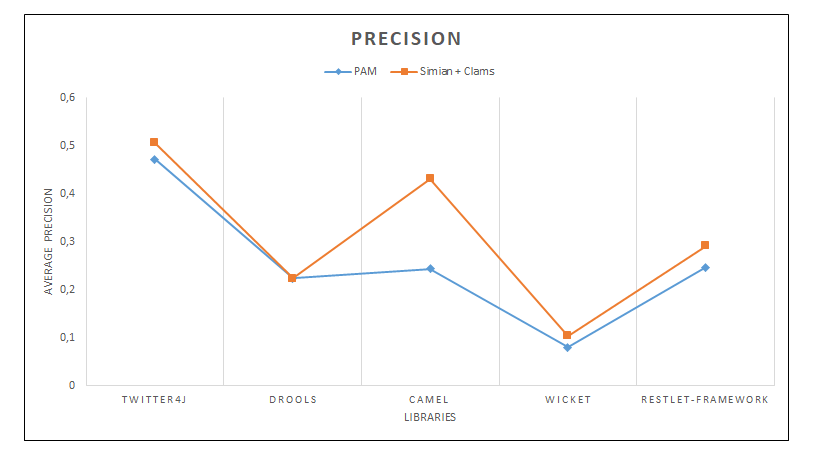
\includegraphics[width=14cm,height=14cm,keepaspectratio]{images/Precision.png}
\centering
  \caption{Precision comparison}
  \label{fig:cmd}
\end{figure}

\begin{figure}[!h]
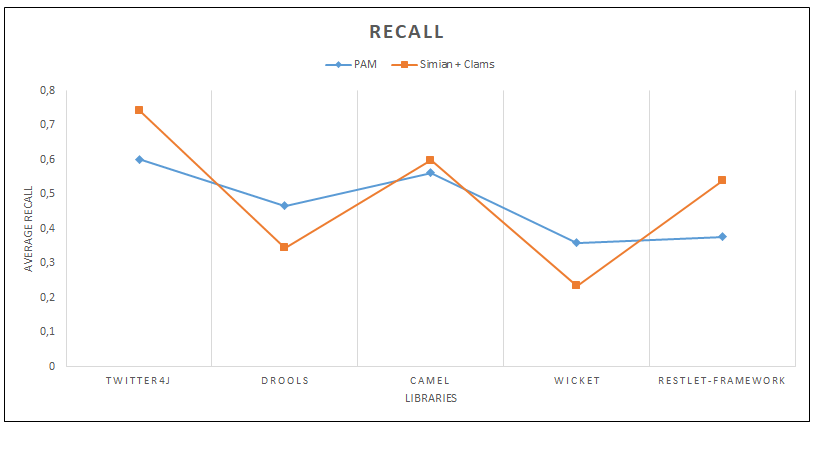
\includegraphics[width=14cm,height=14cm,keepaspectratio]{images/Recall.png}
\centering
\caption{Recall comparison}
\label{fig:cmd}
\end{figure}


\begin{figure}[!h]
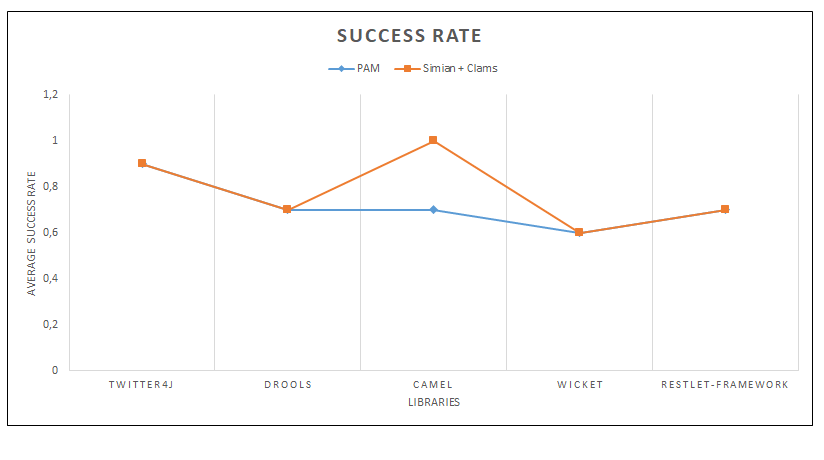
\includegraphics[width=14cm,height=14cm,keepaspectratio]{images/SuccRate.png}
\centering
\caption{Success rate comparison}
\label{fig:cmd}
\end{figure}


\begin{figure}[!h]
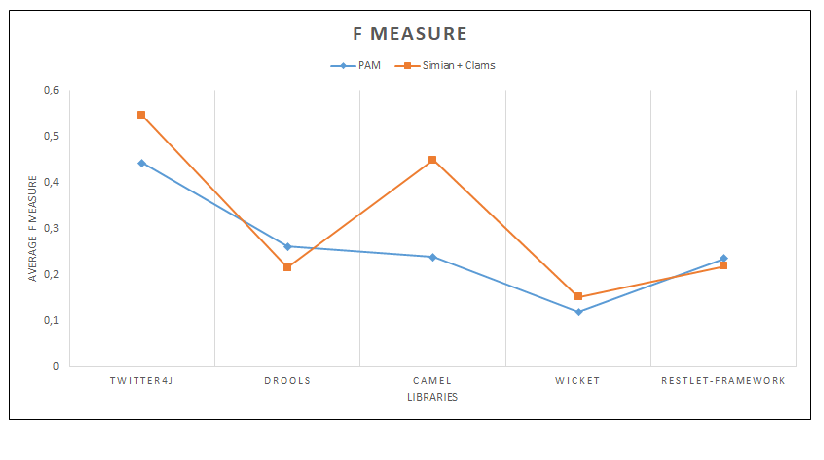
\includegraphics[width=14cm,height=14cm,keepaspectratio]{images/Fmeasure.png}
\centering
\caption{F measure  comparison}
\label{fig:cmd}
\end{figure}


Moreover, we make a time comparison on the computation of the two considered approach, as we pointed out in the \textbf{RQ$_3$}: for PAM, we pick the time needed to produce the list of method invocations starting from a single ARFF file that summarize the context as described before while for our approach, we considered the time needed to produce the recommendations in form of code snippet, considering as context the developer's ground truth (in this case the the ARFF is used by CLAMS to produce the patterns chosen as baseline). The results shows that the time are almost equal,except in the case of wicket library. It happens because PAM relies only on ARFF and, in this case, it contains a huge amount of data. Notice that all the evaluation tasks have been executed on Windows 10 operative system with a Intel core i5-3230M 2.60 GHz processor.

\begin{figure}[!h]
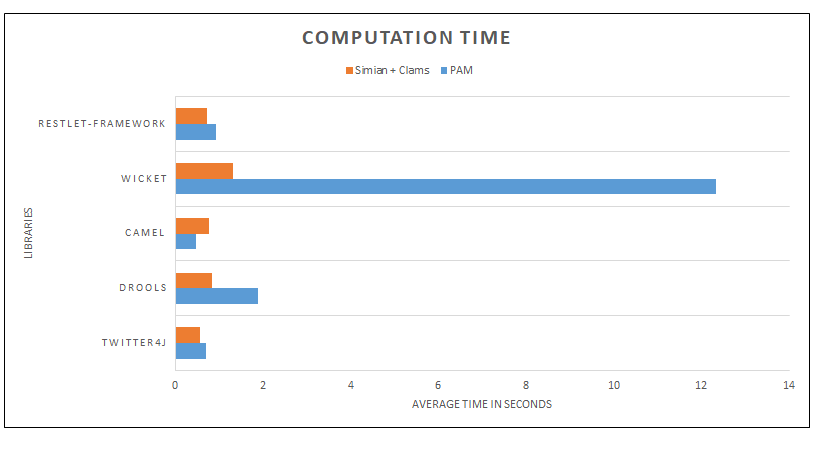
\includegraphics[width=14cm,height=14cm,keepaspectratio]{images/time.png}
\centering
\caption{Time comparison}
\label{fig:cmd}
\end{figure}

The aim of this framework is to give an overall evaluation of accuracy, time, coverage and effectiveness of the proposed approach. The approach relies on the code cloning activity and, so, the results are not immediately comparable with other existing approaches, as they use other techniques like clustering. For this reason, we need this framework to analyze the results in the proper way and to reduce as much as possible bias that can be led from the different domain and techniques. 

	
	
	\chapter{Conclusion}
	\label{sec:conclusion}
	


Aiming to assist developers in their development activities by mining open source software repositories, we propose a framework for providing API function calls. This topic has attracted attention from the research community. Our work is built based on some existing tools and it can be integrated into Eclipse. On the one side, we have Simian, a code cloner that is able to retrieve cloned code among files without needing the pre-processing or post-processing phases. On the other hand, we have CLAMS, a tool that gives as output a ranked list of patterns. The final goal is to provide API function call recommendations in the context of software complex system. This means that we have to analyze Java user's file put within a more bigger structure (as Eclipse project for example). So, a code cloner tool is not enough to generate proper recommendations at the level of code snippet and we integrate the concept of patterns thanks to CLAMS approach. From this, we reuse output files that contain useful patterns for our purposes. In this way, we provide recommendations at level of code snippet, which is closer to code and helps developers complete.%or to have a possible different implementation of the feature that he is developing. Notice that the provided recommendations are always related to a certain library at once. 

%Our approach leaves some open issues. %, those are strongly related with the API recommendations.

From the evaluation framework, it can be seen that the approach is strongly related to the developer's code snippet that Simian takes as input. From the comparison with PAM, we notice that the proposed approach can produce accurate recommendations. Only in the case of some values of recall and f-measure are inferior to those of than PAM. Another issue is that CLAMS patterns have a structure composed first by a list of variable used by the method calls and then the chain of method declaration to realize a specific feature. This structure may introduce some bias because Simian can find similarities only among the list of variables and not in the method calls. Moreover, Simian divides source code to analyze into blocks, limited by the threshold parameter. In some cases this can lead to false positives since Simian cannot identify a certain pattern in the code if it is not smaller than the threshold value. For example, in source code there are two methods that belong to a CLAMS pattern which includes another method invocations, if in the original source code the third invocation differs from that, Simian is not able to retrieve the pattern. Some threats could arise from the evaluation framework in which we used Rascal. In order to validate the approach, we had set up an Eclipse structure as shown in the related section. Although the structure is correct, it is manually built so it may affect the metrics, in particular precision and recall.
 
%From the point of view of improvements, 

We opt for a code cloner, however there are a lot of alternative approaches that can be exploited, like another code cloner or change completely the approach. We can beautify the output results that are presented in a simple file by setting up an Eclipse plugin, with all necessary components. Regarding the evaluation, we can provide a human survey by involving developers with different skills and knowledge to asses the provided results with a different perspective. Considering other approaches, many studies use probabilistic techniques, for example, define models or probability distribution. The central point of our work is the use of a code cloner to detect similarities between the pattern retrieved by CLAMS and the actual code snippet. Although Simian doesn't have any pre- or post-processing phases, we overcome this limitations by manually selecting source files and ranking the results, considering the duplicated lines of code. Moreover, we added also the AST concept in the evaluation framework. In this way, we are able to equip Simian with a new functionality that considers only the textual similarity. %Following this road, a possible improvement should be use a code cloner based on different similarity comparison (like suffix tree), but the challenge of integrate it in the Eclipse platform still remain opened. Most of code cloner are developed for simply analyze the developer's code and are used only to find clones in different files.   

%For future work, we are going to thoroughly evaluate our proposed approach by using other similar techniques as baseline, with the consideration of more data.

%. In this work we presented our proposed approach to deal with API recommendations
%As the precision of the mined code snippets (like false positive in the Simian analysis or in the CLAMS patterns). 
	\newpage
	
	
	
	%----------------------------------------------------------------------------------------
	%	THESIS CONTENT - APPENDICES
	%----------------------------------------------------------------------------------------
	
	\appendix % Cue to tell LaTeX that the following "chapters" are Appendices
	
	% Include the appendices of the thesis as separate files from the Appendices folder
	% Uncomment the lines as you write the Appendices
	
	\include{src/AppendixA}
	
	%----------------------------------------------------------------------------------------
	%	BIBLIOGRAPHY
	%----------------------------------------------------------------------------------------
	
	\printbibliography[heading=bibintoc]
	
	%----------------------------------------------------------------------------------------
	
\end{document}  
